\documentclass[t]{beamer}  % [t], [c], или [b] --- вертикальное выравнивание на слайдах (верх, центр, низ)

% \documentclass[t]{beamer}  % [t], [c], или [b] --- вертикальное выравнивание на слайдах (верх, центр, низ)
%\documentclass[handout]{beamer} % Раздаточный материал (на слайдах всё сразу)
%\documentclass[aspectratio=169]{beamer} % Соотношение сторон

\usetheme{Berlin} % Тема оформления
%\usetheme{Madrid}
%\usetheme{Frankfurt}
%\usetheme{CambridgeUS}

\usecolortheme{albatross} % Цветовая схема
%\usecolortheme{monarca} % Цветовая схема
%\usecolortheme{fly} % Цветовая схема
%\useinnertheme{circles}
%\useinnertheme{rectangles}

%\usetheme{HSE}

%%% Работа с русским языком
\usepackage{cmap}					% поиск в PDF
\usepackage{mathtext} 				% русские буквы в формулах
\usepackage[T2A]{fontenc}			% кодировка
% \usepackage[utf8]{inputenc}			% кодировка исходного текста
\usepackage[english,ukrainian]{babel}	% локализация и переносы
\usepackage{amsmath}
\usepackage{amsfonts}
\usepackage{amssymb}

\usepackage{hyperref}

%%% Работа с картинками
\usepackage{graphicx}  % Для вставки рисунков
\graphicspath{{images/}{images2/}}  % папки с картинками
\setlength\fboxsep{3pt} % Отступ рамки \fbox{} от рисунка
\setlength\fboxrule{1pt} % Толщина линий рамки \fbox{}
\usepackage{wrapfig} % Обтекание рисунков текстом

%%% Работа с таблицами
\usepackage{array,tabularx,tabulary,booktabs} % Дополнительная работа с таблицами
\usepackage{longtable}  % Длинные таблицы
\usepackage{multirow} % Слияние строк в таблице

%%% Программирование
\usepackage{etoolbox} % логические операторы

%%% Другие пакеты
\usepackage{lastpage} % Узнать, сколько всего страниц в документе.
\usepackage{soul} % Модификаторы начертания
\usepackage{csquotes} % Еще инструменты для ссылок
%\usepackage[style=authoryear,maxcitenames=2,backend=biber,sorting=nty]{biblatex}
\usepackage{multicol} % Несколько колонок

%%% Картинки
\usepackage{tikz} % Работа с графикой
\usepackage{pgfplots}
\usepackage{pgfplotstable}

\title[Python]{Мова програмування Python для початківців}
%\subtitle{За матеріалами "Системне адміністрування Linux" Сергія Клочкова}
\author{Легенький М.М.}
\date{\today}
\institute[Факультет радіофізики, біомедичної електроніки та комп'ютерних систем]{Факультет радіофізики, біомедичної електроніки та комп'ютерних систем}

\setbeamertemplate{caption}[numbered]

\titlegraphic { 
\begin{tikzpicture}[overlay,remember picture]
\node[left=0.2cm] at (current page.32){
    
\includegraphics[width=3cm]{rbecs_logo}
};
\node[right=0cm] at (current page.148){
    
\includegraphics[width=1.5cm]{python_logo}
};
\end{tikzpicture}
}

\logo{
\begin{tikzpicture}[overlay,remember picture]
\node[left=0cm] at (current page.-26){
    
\includegraphics[width=3cm]{rbecs_logo}
};
\node[right=0cm] at (current page.-153){
    
\includegraphics[width=1.5cm]{python_logo}
};
\end{tikzpicture}}


% \includeonly{presentaion2} 
%\includeonly{file2,file3} % пробела после запятой быть не должно

\begin{document}

\frame[plain]{\titlepage}	% Титульный слайд

\begin{frame}{План лекції}
    \tableofcontents
\end{frame}

% \section*{Лекція 1: Знайомство з Python}
 
\subsection{Вступ}
\begin{frame}
\frametitle{Викладач}
\begin{wrapfigure}{r}{0.35\textwidth}

\includegraphics[width=0.25\textwidth]{pictures/myphoto}
\caption{Легенький М.М.}
\label{myphoto}
\end{wrapfigure}
\textbf{Легенький Максим Миколайович}

доцент кафедри теоретичної радіофізики

\textit{факультету радіофізики, біомедичної електроніки та комп’ютерних систем}

aуд. 5-5

тел. (057) 707-52-57

e-mail: \href{mailto:mlegenkiy@karazin.ua}{mlegenkiy@karazin.ua}

Telegram: \href{https://t.me/mlegenkiy}{@mlegenkiy}
\end{frame}

\begin{frame}
\frametitle{Мотивація}
\begin{itemize}
   \item Комп'ютерна грамотність — оволодіння мінімальним набором знань і навичок роботи на персональному комп'ютері. 
  \item Нині комп'ютерна грамотність —  вміння, таке ж необхідне, як і вміння читати й писати. 
   \item Що робити ? Вивчати Python!
\end{itemize}
\end{frame}

\subsection{Що таке Python?}
\begin{frame}
\frametitle{Python}
% 	\frametitle{\insertsection} 
% 	\framesubtitle{\insertsubsection}
\begin{wrapfigure}{r}{0.35\textwidth}
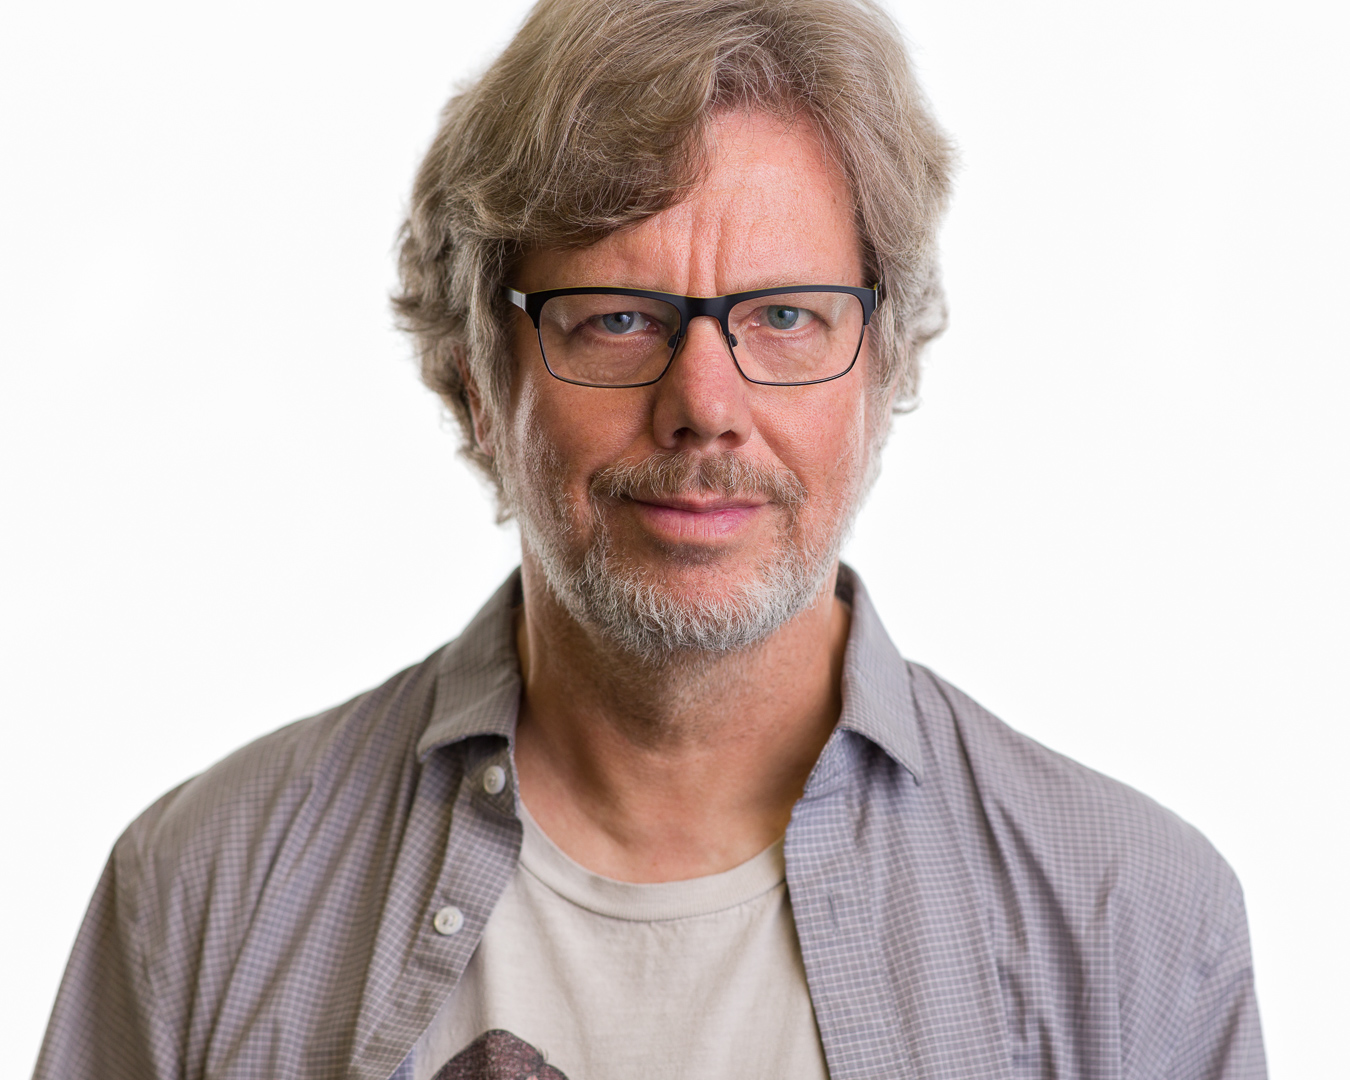
\includegraphics[width=0.25\textwidth]{pictures/guido}
\caption{Гвідо ван Россум}
\label{gvido}
\end{wrapfigure}
Python (Пайтон) — інтерпретована об'єктно-орієнтована мова програмування високого рівня зі строгою динамічною типізацією.  Назву запозичено із назви британського шоу Монті Пайтон. Розроблена в 1990 році Гвідо ван Россумом. 
\end{frame}

\begin{frame}
\frametitle{Версії Python}
%\begin{wrapfigure}{r}{0.35\textwidth}
\begin{figure}
  \begin{center}
    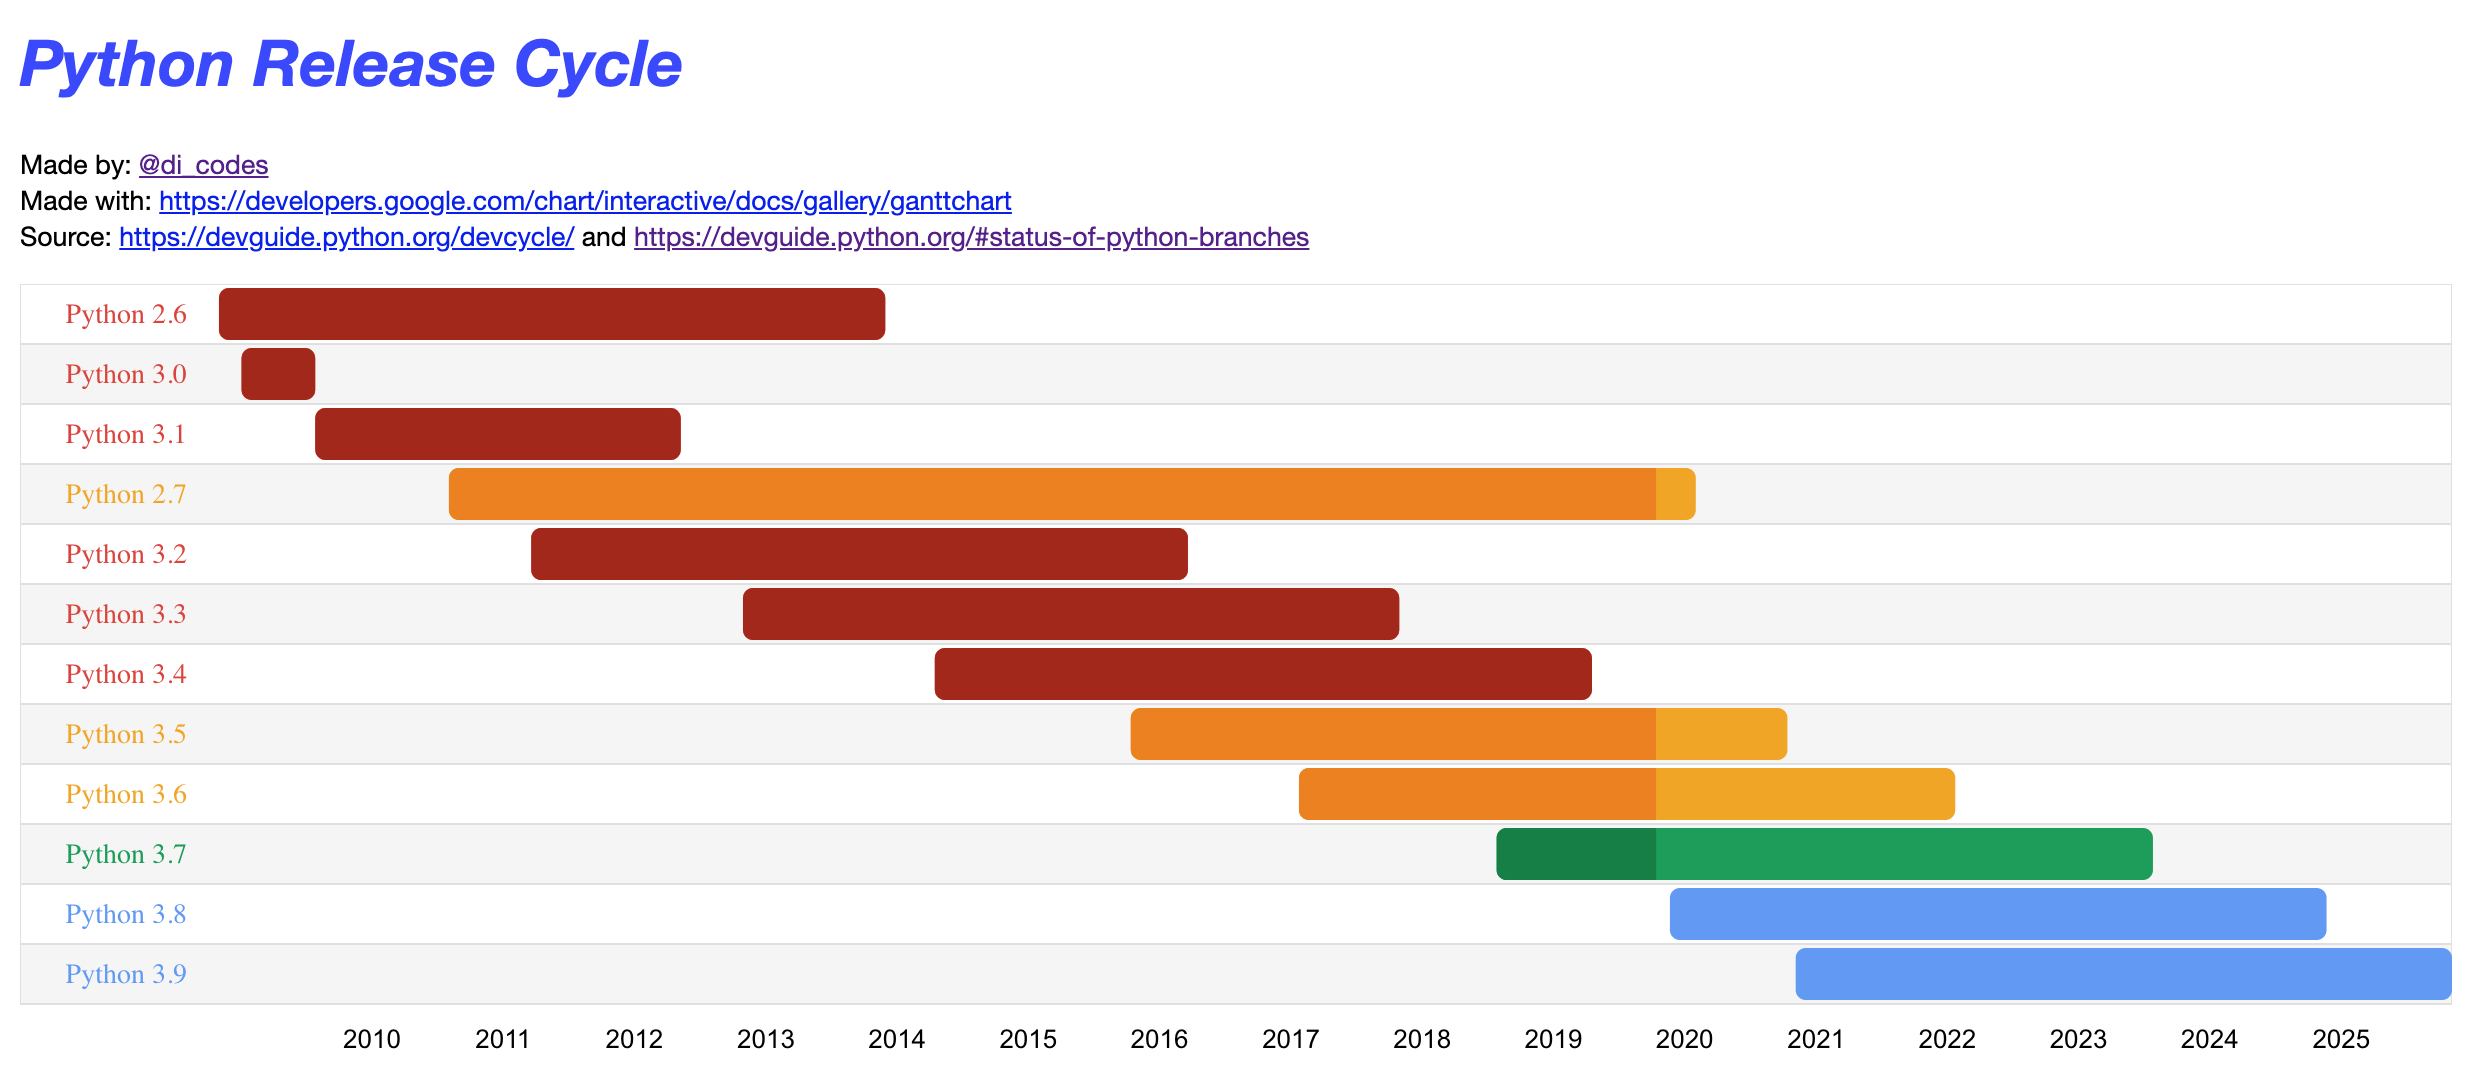
\includegraphics[width=\textwidth,height=0.5\textheight]{pictures/python_versions}
  \caption{Версії Python та період їх підтримки}
\label{versions}
  \end{center}
\end{figure}
\end{frame}

\begin{frame}
\frametitle{Переваги та недоліки Python}
Переваги:
\begin{itemize}
  \item зручність та простота програмування;
  \item переносимість програм;
  \item велика кількість модулів;
  \item поширеність та популярність.
\end{itemize}
Недоліки:
\begin{itemize}
  \item порівняно низька швидкість виконання програм;
  \item неможливість модифікації вбудованих класів.
\end{itemize}
\end{frame}

\begin{frame}
\frametitle{Переваги та недоліки Python}
\begin{itemize}
  \item Python  застосовується при розробці алгоритмів штучного інтелекту (в нейронних мережах);
  \item Python  застосовується при розробці серверної частини сайтів за допомогою Django та Flask (Instagram, YouTube, алгоритми пошуку Google, Dropbox, тощо);
  \item Python  застосовується в наукових проєктах та для обробки даних (Big Data);
  \item Python  застосовується для Web Parsing.
\end{itemize}
\end{frame}


\begin{frame}
\frametitle{Зручність та простота коду Python}
\begin{figure}
\begin{center}
 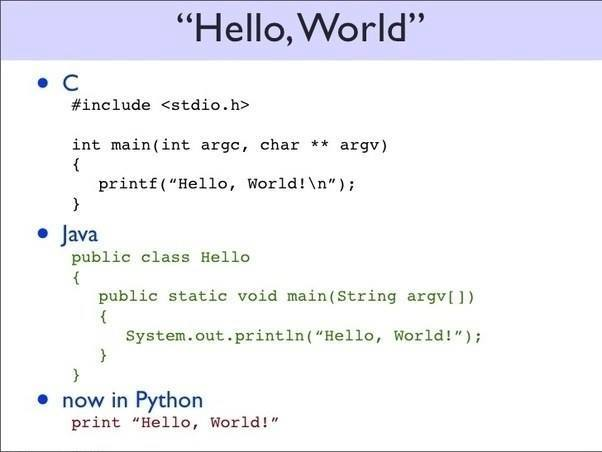
\includegraphics[width=0.4\textwidth]{pictures/helloworld.png}
\caption{Код на C, Java та Python для виведення на екран рядку "Hello, World!"}
\label{python_site} 
\end{center}
\end{figure}
\end{frame}

\begin{frame}
\frametitle{Python має велику кількість бібліотек та фреймворків}
\begin{figure}
\begin{center}
 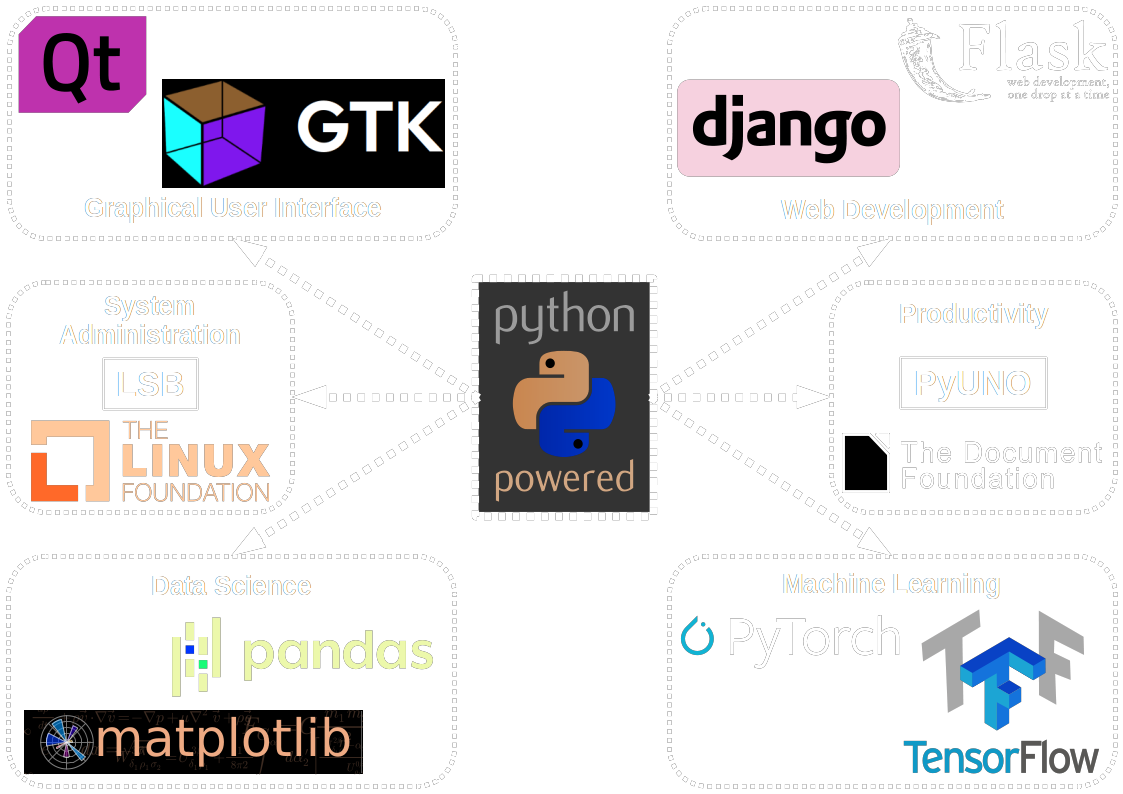
\includegraphics[width=0.6\textwidth]{pictures/python_frameworks1.png}
\caption{Фреймворки Python}
\label{python_site} 
\end{center}
\end{figure}
\end{frame}

\begin{frame}
\frametitle{Python є однією із найпопулярніших мов програмування}
\begin{figure}
\begin{center}
 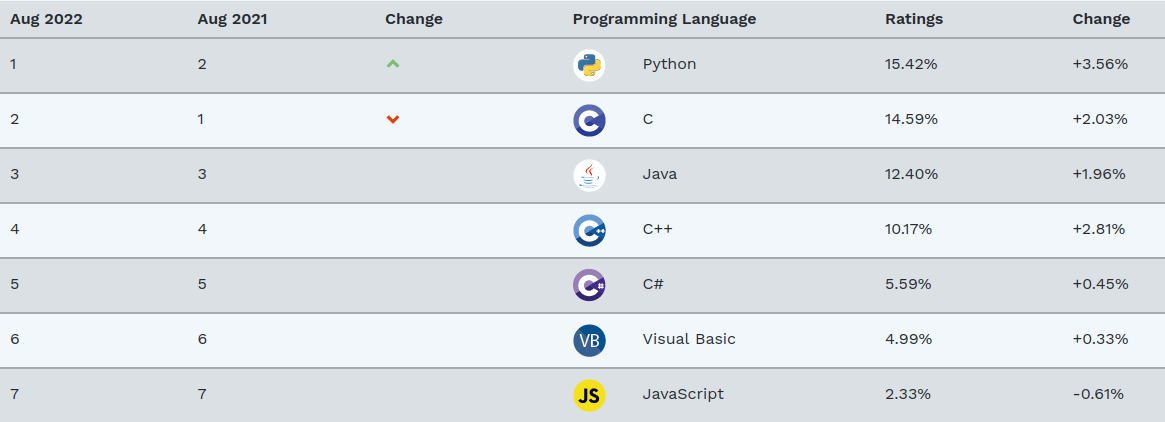
\includegraphics[width=0.6\textwidth]{pictures/tiobe.png}
\caption{З сайту \href{https://www.tiobe.com/tiobe-index/}{TIOBE}}
\label{python_site} 
\end{center}
\end{figure}
\tiny{TIOBE індекс (рейтинг мов програмування) — показник популярності мов програмування. Розраховується виходячи з кількості результів запитів до пошукових систем, що містять назву мови. Охоплює пошуки в Google, MSN, Yahoo!, Baidu, Вікіпедії і Youtube.}
\end{frame}



\subsection{Робота з Python}
\begin{frame}
\frametitle{Сайт Python}
\begin{figure}
\begin{center}
 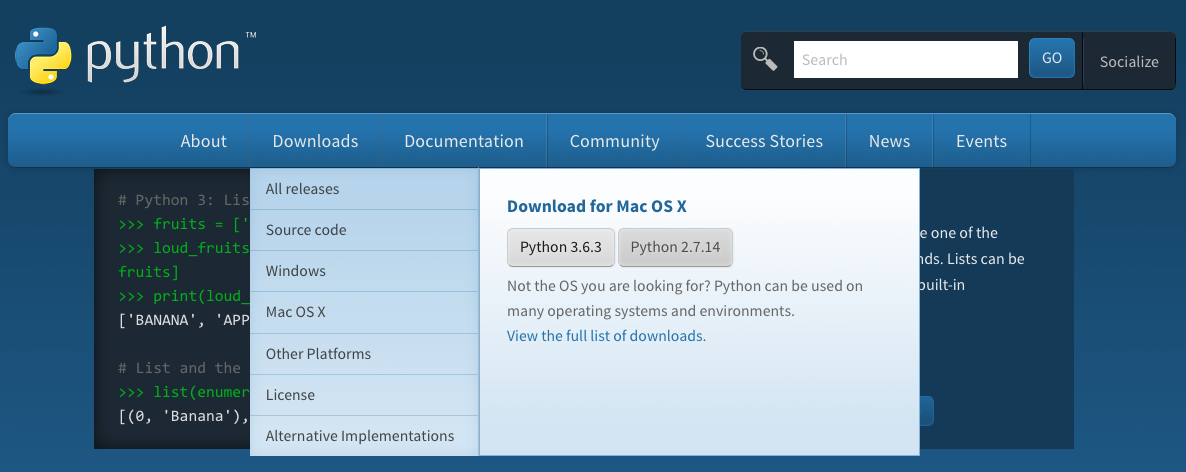
\includegraphics[width=0.95\textwidth]{pictures/python_site.png}
\caption{Сайт: \href{https://python.org/}{python.org}}
\label{python_site} 
\end{center}
\end{figure}

\end{frame}

\begin{frame}
\frametitle{Встановлення Python}
\begin{figure}
\begin{center}
 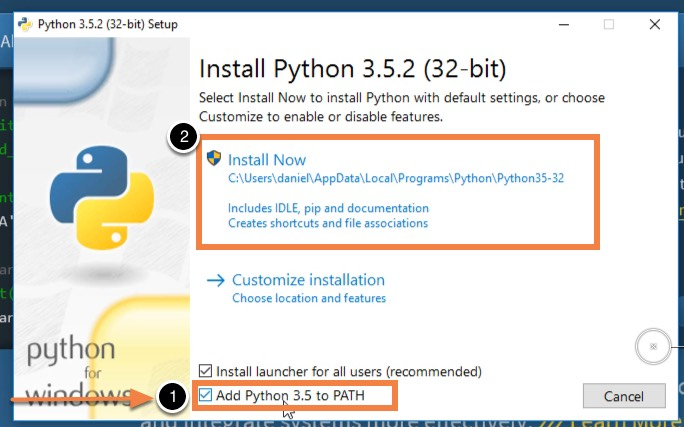
\includegraphics[width=0.4\textwidth]{pictures/python_install.jpg}
\caption{Встановлення Python}
\label{python_install} 
\end{center}
\end{figure}
\tiny{\href{https://uk.wikibooks.org/wiki/}{uk.wikibooks.org/wiki/Пориньте\_у\_Python\_3/Встановлення} - інструкція зі встановлення Python.}
\end{frame}

\begin{frame}
\frametitle{Виконання коду Python}

\begin{wrapfigure}{l}{0.45\textwidth}
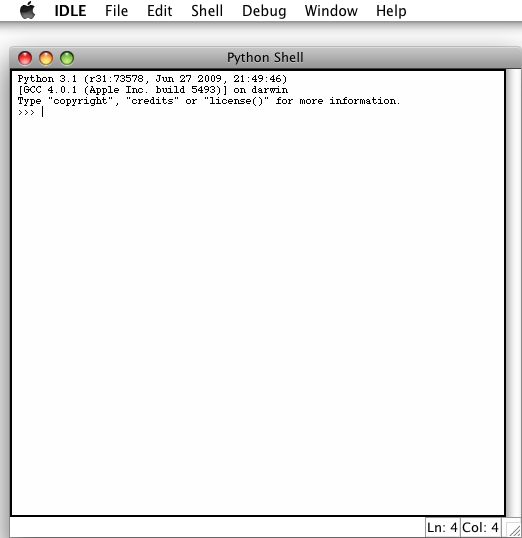
\includegraphics[width=0.35\textwidth]{pictures/idle.png}
\caption{IDLE}
\label{myphoto}
\end{wrapfigure}

Код Python може виконуватися в \textit{інтерактивному} та \textit{файловому} режимі.
\end{frame}


\begin{frame}
\frametitle{Виконання коду Python}
\href{https://it-need.com/pep-8-posibnyk-z-napysannya-kodu-na-python/}{PEP8} містить перелік принципів написання красивого та лаконічного програмного коду мовою Python (PEP – Python Enhancement Proposal, пропозиції щодо розвитку Python).
\begin{figure}
\begin{center}
 
\includegraphics[width=0.5\textwidth]{pictures/pep8.png}
\caption{PEP8}
\label{python_site} 
\end{center}
\end{figure}
\end{frame}

\begin{frame}
\frametitle{PyCharm}


\begin{wrapfigure}{r}{0.4\textwidth}

\includegraphics[width=0.25\textwidth]{pictures/pycharm_logo.png}
\caption{Логотип PyCharm}
\label{pycharm_logo}
\end{wrapfigure}

\textbf{PyCharm} — інтегроване середовище розробки для мови програмування Python. \href{https://www.jetbrains.com/pycharm/download/}{Сайт} для завантаження PyCharm.
\end{frame}


\subsection{Організація курсу}
\begin{frame}
\frametitle{Структура курсу}
\end{frame}

% \section{Лекція 2: Математика в Python}
 
\begin{frame}
\frametitle{Дані в Python}
\begin{itemize}
  \item Змінна - посилання на об'єкт
  \item Оператор присвоювання: 
  
  \texttt{Операнд зліва = Операнд зправа}
  \item Динамічна типізація
  \item \texttt{a = 7; b = a}
  \item Каскадне присвоювання: \texttt{a = b = c = 0}
  \item Множинне присвоювання: \texttt{a, b = 1, 2}
  \item Обмін значеннями: \texttt{a, b = b, a}
\end{itemize}
\end{frame}

\begin{frame}
\frametitle{Функція id}
Функція id(object) повертає «ідентифікаційний номер» об'єкта object, який є унікальним та незмінним.
\begin{figure}
\begin{center}
 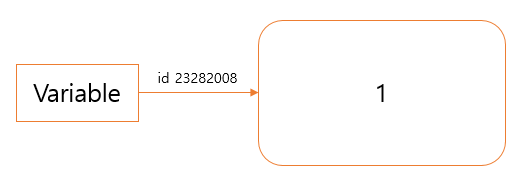
\includegraphics[width=0.7\textwidth]{pictures/id_func.png}
\caption{Функція id}
\label{id} 
\end{center}
\end{figure}
\end{frame}

\begin{frame}
\frametitle{Функція type}
Функция type(object) повертає тип об'єкту object. Його значення таке ж, як у змінної екземпляру object .\_\_ class\_\_.
\begin{figure}
\begin{center}
 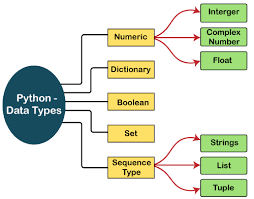
\includegraphics[width=0.5\textwidth]{pictures/python_data_types.png}
\caption{Типи даних в Python}
\label{data_types} 
\end{center}
\end{figure}
\end{frame}


\begin{frame}
\frametitle{Імена змінних}
\begin{itemize}
  \item Перший символ - будь-яка літера латинського алфавіту a-z, A-Z та символ підкреслення \_. Інші символи - теж саме та цифри 0-9.
  \item Іменами слід обирати іменники.
  \item Імена повинні відображати сенс даних.
  \item Неможна використовувати зарезервовані слова (Pycharm - Python Console - help() - keywords).
  \item Не слід використовувати імена вбудованих функцій.
\end{itemize}
\end{frame}
 
\begin{frame}
\frametitle{Типи чисел в Python}
\begin{itemize}
  \item цілі числа (int);
  \item дійсні числа (float);
  \item комплексні числа (complex).
\end{itemize} 
  
\end{frame}

 
\begin{frame}
\frametitle{Арифметичні операції}

\begin{table}
  \caption{Арифметичні операції}
  \label{tab:}

  \begin{center}
    \begin{tabular}{|c|c|c|}
      \hline
      \textbf{Оператор} & \textbf{Опис} & \textbf{Пріоритет} \\
      \hline
      + & додавання & 2 \\
       \hline
      - & віднімання & 2 \\
       \hline
      * & множення & 3 \\
       \hline
       /,// & ділення & 3 \\
       \hline
       \% & залишок від ділення & 3 \\
       \hline
       ** & піднесення в ступінь & 4 \\
       \hline
    \end{tabular}
  \end{center}
\end{table}
 \begin{center}
   \tiny{// - ділення з округленням до найменшого цілого}
  \end{center}
\end{frame}

\begin{frame}
\frametitle{Скорочені оператори в Python}
Оператор += додає значення правого операнда до лівого та присвоює цю суму лівому операнду.

Аналогічно працюють оператори -=, *=, /=, \%=, **=, //=.  
\end{frame}


\begin{frame}
\frametitle{Математичні функції}
\begin{itemize}
  \item abs(a)
  \item min(a, b, ...)
  \item max(a, b, ...)
  \item pow(a, b)
  \item round(a)
  \item round(a, n)
\end{itemize} 
  
\end{frame}

\begin{frame}
\frametitle{Модуль math}
Для того щоб звернутися до функцій модулю math, спочатку треба імпортувати цей модуль командою \texttt{import math}.
\begin{figure}
\begin{center}
 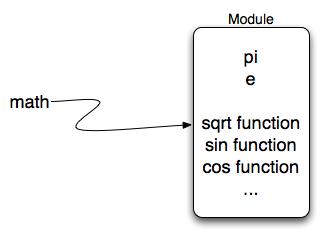
\includegraphics[width=0.5\textwidth]{pictures/mathmod.png}
\caption{Модуль math}
\label{mathmodule} 
\end{center}
\end{figure}
\end{frame}

\begin{frame}
\frametitle{Функції print та input}
\begin{itemize}
  \item print - вивід даних в консоль
      \begin{itemize}
        \item sep - роздільник між даними
        \item end - останній символ (символи)
     \end{itemize} 
  \item input - ввід даних зі стандартного вхідного потоку (клавіатури)
      \begin{itemize}
        \item int(input())
        \item float(input())
     \end{itemize}
 \end{itemize} 
\end{frame}

% \section*{Лекція 3: Рядки}
\subsection{Створення рядків у Python} 
\begin{frame}
\frametitle{Рядки}
Рядок - упорядкований набір символів. Рядок - незмінний тип даних.
\begin{figure}
\begin{center}
 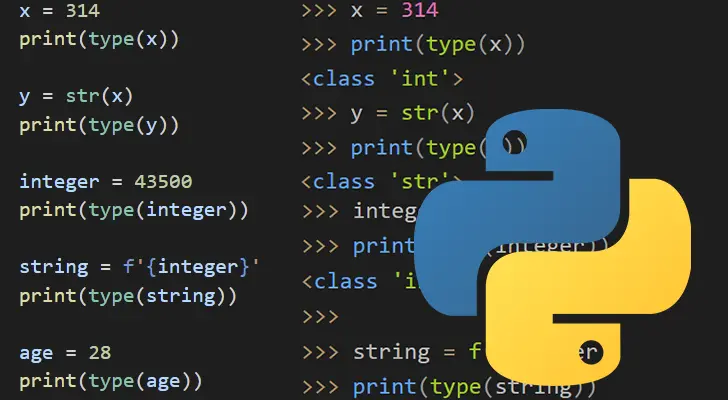
\includegraphics[width=0.6\textwidth]{pictures/strings.png}
\caption{Рядки у Python}
\label{python_site} 
\end{center}
\end{figure}
\end{frame}

\begin{frame}
\frametitle{Створення рядків}
\begin{itemize}
  \item В одинарних лапках 'Python'
  \item В подвійних лапках "Python"
  \item 
  В потрійних лапках '''Python
  
  is the best!'''
  \item Символ переноса рядка \textbackslash n
 \end{itemize}
\begin{figure}
\begin{center}
 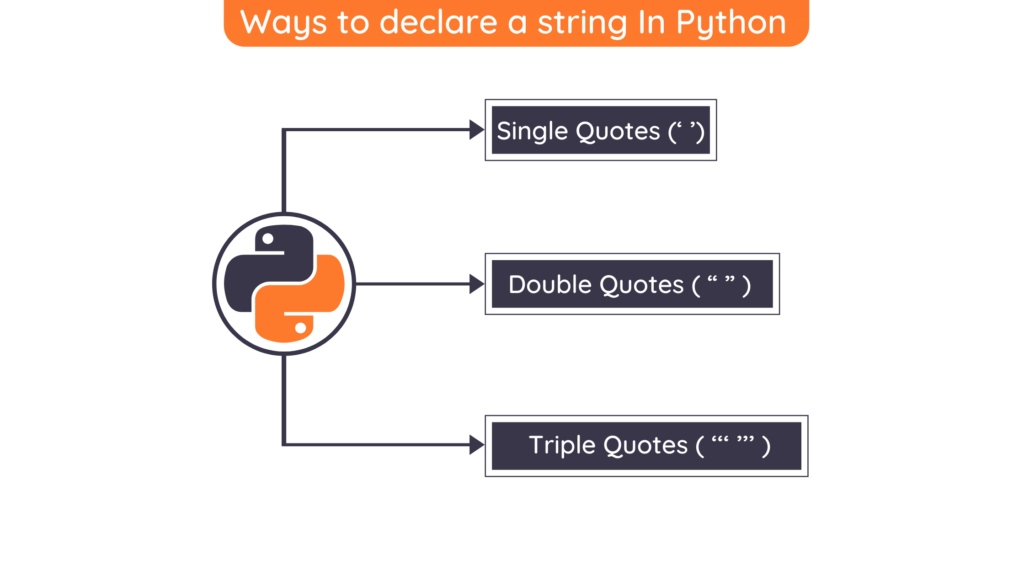
\includegraphics[width=0.4\textwidth]{pictures/declare_string.png}
\caption{Створення рядків у Python}
\label{python_site} 
\end{center}
\end{figure}
\end{frame}

\subsection{Операції над рядками} 
\begin{frame}
\frametitle{Операції над рядками}
\begin{itemize}
  \item Конкатенація рядків (оператор \texttt{+})
  \item Повторення рядків (оператор \texttt{*})
  \item Функція \texttt{str}
  \item Довжина рядка. Функція \texttt{len}
  \item Оператор входження \texttt{in}
 \end{itemize}

\end{frame}

\begin{frame}
\frametitle{Порівняння рядків}
\begin{itemize}
  \item Дорівнює \texttt{==} або не дорівнює \texttt{!=}.
  \item Більше \texttt{>} або менше \texttt{<}.
  \item Функції \texttt{ord} та \texttt{chr}.
\end{itemize}
\begin{figure}
\begin{center}
 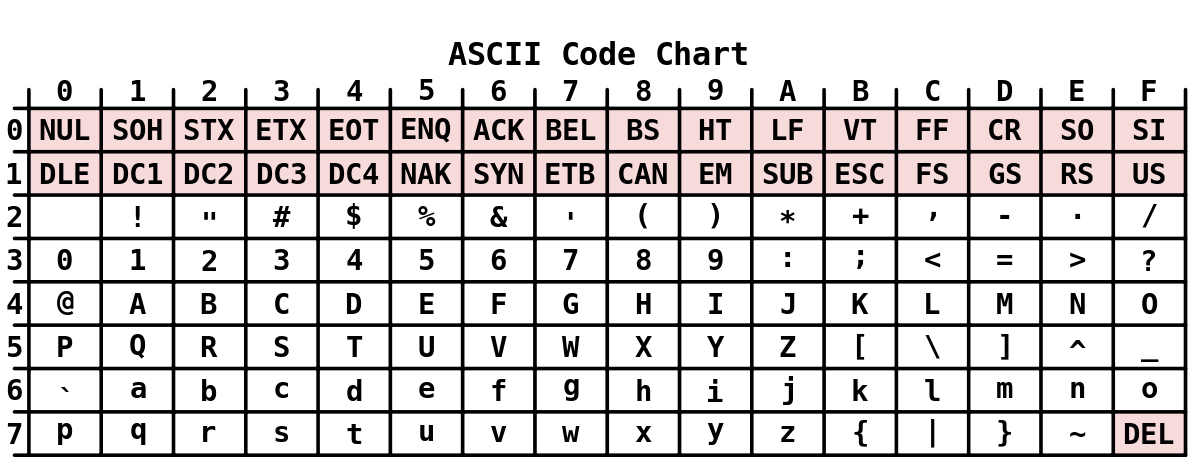
\includegraphics[width=0.7\textwidth]{pictures/ASCII-Table.png}
\caption{Таблиця ASCII}
\label{ASCII-Table} 
\end{center}
\end{figure}
\end{frame}

\begin{frame}
\frametitle{Елементи рядків}
Щоб отримати  i-й елемент рядка s використовується конструкція s[i]. Індекс i змінюється від 0 до len(s) - 1 (або від -1 до -len(s)).
\begin{figure}
\begin{center}
 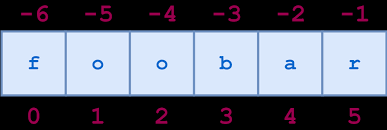
\includegraphics[width=0.5\textwidth]{pictures/string.png}
\caption{Елементи рядка}
\label{string} 
\end{center}
\end{figure}
\end{frame}

\begin{frame}
\frametitle{Зріз рядка}
Зріз (slice) — витяг із рядка одного символу або деякого фрагмента підрядка чи підпослідовності.

\begin{center}
\LARGE{s[start:stop:step]}
\end{center}
\end{frame}

\subsection{Методи рядків} 

\begin{frame}
\frametitle{Методи}
\begin{center}
\texttt{об'єкт.метод(аргументи)}
\end{center}
\begin{figure}
\begin{center}
 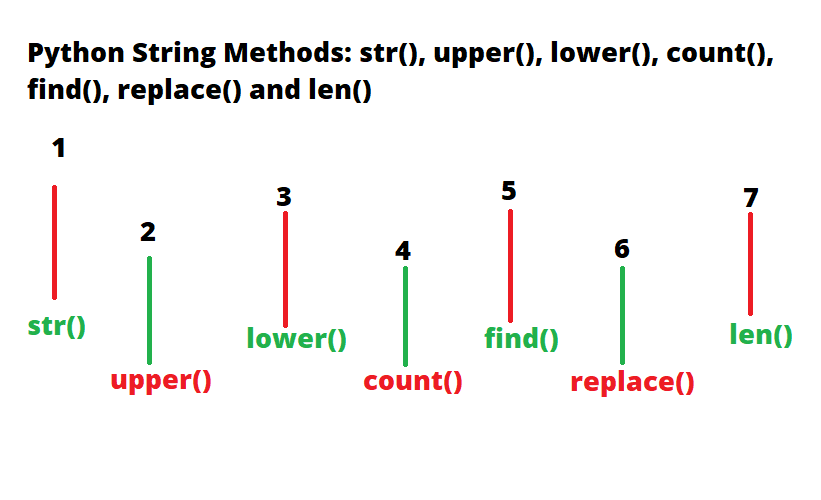
\includegraphics[width=0.5\textwidth]{pictures/python-string-methods.png}
\caption{Методи рядків}
\label{python-string-methods} 
\end{center}
\end{figure}
\end{frame}

\begin{frame}
\frametitle{Методи рядка s}
\begin{itemize}
  \item s.upper() - перетворює всі маленькі літери у великі;
  \item s.lower() - перетворює всі великі літери в маленькі;
  \item s.count(sub[, start[, end]]) - підрахунок кількості підрядків в рядку;
  \item s.find(sub[, start[, end]]) - індекс першого входження підрядка в рядку (find - пошук зліва направо, rfind - пошук зправа наліво);
  \item s.index(sub[, start[, end]]) - аналогічно до find, в разі не знаходження повертає помилку (find повертає -1);
\end{itemize}
\end{frame}

\begin{frame}
\frametitle{Методи рядка s}
\begin{itemize}
 \item s.replace(old, new[, count=-1]) - заміна підрядка old на підрядок new (count - кількість замін, count = -1 - без обмежень);
 \item s.isalpha() - повертає істину якщо рядок повністю складається із літер (інакше -повертає брехню);
 \item s.isdigit() - повертає істину якщо рядок повністю складається із цифр (інакше -повертає брехню);
 \item s.rjust(width[, fillcar=' ']) - повертає рядок заданої ширини width, fillcar - символи, що за потреби додаються зліва (у функції ljust - зправа);
\end{itemize}
\end{frame}

\begin{frame}
\frametitle{Методи рядка s}
\begin{itemize}
 \item s.split(sep=None, maxsplit=-1) - розбиває рядок за вказаним символом sep;
 \item s.join(list) - поєднує елементи списка list через роздільник s;
 \item s.strip(list) - видаляє всі символи пропусків та переносів рядків напочатку та вкінці рядка (rstrip - тільки зліва, lstrip - тільки зправа).
\end{itemize}
\end{frame}

\subsection{Спеціальні символи та методи формування рядків}

\begin{frame}
\frametitle{Спеціальні символи рядків}
\tiny{
\begin{table}
  \caption{Спеціальні символи}
  \label{tab:}

  \begin{center}
    \begin{tabular}{|p{1.2cm}|p{3.5cm}|p{1.2cm}|p{3.5cm}|}
    \hline
     \textbf{Позначення}  & \textbf{Опис} & \textbf{Позначення}  & \textbf{Опис} \\
     \hline
      \textbackslash n & Перевод рядка & \textbackslash \textbackslash & Символ зворотнього слеша \\
     \hline
           \textbackslash ' & Символ апострофа & \textbackslash " & Символ подвійної лапки \\
     \hline
           \textbackslash a & Звуковий сигнал & \textbackslash b & Емуляція клавіші BackSpace \\
     \hline
           \textbackslash f & Переклад формату & \textbackslash r & Повернення каретки \\
     \hline
           \textbackslash t & Горизонтальна табуляція (4 пропуски) & \textbackslash v & Вертикальна табуляція \\
     \hline
           \textbackslash 0 & Символ Null (не признак кінця рядка) & \textbackslash xhh & Символ з шістнадцятковим кодом hh \\
     \hline
           \textbackslash ooo & Символ з вісімковим кодом ooo  & \textbackslash N\{id\} & Ідентифікатор із кодової таблиці Unicode \\
     \hline
           \textbackslash uhhhh & 16-ти бітний символ Unicode в шістнадцятковій формі & \textbackslash Uhhhhhhhh &  32-х бітний символ Unicode в шістнадцятковій формі\\
     \hline
    \end{tabular}
  \end{center}
\end{table}
}
\end{frame}

\begin{frame}
\frametitle{"Сирі" (raw) рядки}
Якщо перед рядком поставити літеру \texttt{r}, то всі символи в ньому будуть сприйматися так, як вони написані.
\begin{figure}
\begin{center}
 
\includegraphics[width=\textwidth]{pictures/raw_string.png}
\caption{Приклад сирого рядка}
\label{raw_string} 
\end{center}
\end{figure}
\end{frame}

\begin{frame}
\frametitle{Методи формування рядків}
name = "Bruce"

age = 35
\begin{itemize}
  \item "My name is " + name + " and my age is " + str(age)
  \item "My name is \{0\} and my age is \{1\}".format(name, age)
  \item "My name is \{fio\} and my age is \{old\}".format(fio=name, old=age)
  \item f"My name is \{name\} and my age is \{age\}"
\end{itemize}
\end{frame}

% \section*{Лекція 4: Списки}
\subsection{Списки та операції над ними} 
\begin{frame}
\frametitle{Створення списків у Python}
Список - впорядкована колекція даних різних типів.

Список відноситься до змінних типів даних.

Пустий список - []. Для створення списку на основі об'єкту, який можна перебирати, використовується функція list.
\begin{figure}
\begin{center}
 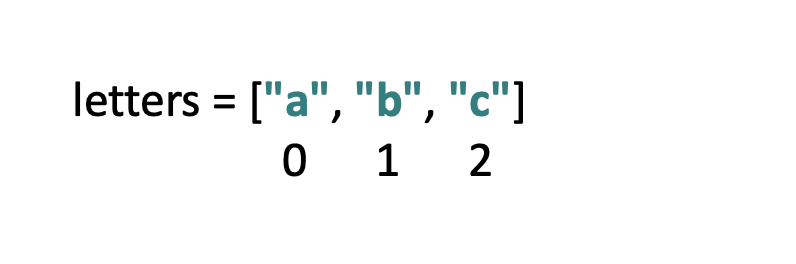
\includegraphics[width=0.6\textwidth]{pictures/list.png}
\caption{Список}
\label{list} 
\end{center}
\end{figure}

\end{frame}

 
\begin{frame}
\frametitle{Основні  функції для роботи зі списком s}
    \begin{itemize}
        \item<1-> \texttt{len(s)} - визначення числа елементів у списку;
        \item<2-> \texttt{max(s)} - знаходження максимального значення;
        \item<2-> \texttt{min(s)} - знаходження мінімального значення;
        \item<3-> \texttt{sum(s)} - розрахунок суми;
        \item<4-> \texttt{sorted(s)} - сортування за зростанням;
        \item<4-> \texttt{sorted(s, reverse=True)} - сортування за спаданням.
    \end{itemize}
\end{frame}

\begin{frame}
\frametitle{Оператори для роботи зі списками}
    \begin{itemize}
        \item<1-> \texttt{+} - поєднання двох списків в один;
        \item<2-> \texttt{*} - повторення списку;
        \item<3-> \texttt{in} - перевірка входження елементу в список;
        \item<4-> \texttt{del} - видалення елементу списку.
    \end{itemize}
\end{frame}

\subsection{Робота зі списками} 
\begin{frame}
\frametitle{Зрізи}
Зрізи дозволяють отримати деяку підмножину значень списку:
\vspace{1cm}
\begin{center}
\huge{lst[start:stop[:step]]}
\end{center}
\normalsize

\end{frame}


\begin{frame}
\frametitle{Копіювання та порівнювання списків}
Для створення копії списка \texttt{lst} використовується команда \texttt{lst[:]} або \texttt{list(lst)}.

Списки можна лексикографічно порівнювати між собою за допомогою операторів: >, <, == та !=.
\begin{table}
  \caption{}
  \label{tab:}

  \begin{center}
    \begin{tabular}{|c|c|}
    \hline
      \textbf{Оператор} & \textbf{Значення} \\
      \hline
      > & більше \\
      \hline
      < & менше\\
      \hline
      == & дорівнює \\
      \hline
      != & не дорівнює\\
      \hline
    \end{tabular}
  \end{center}
\end{table}
\end{frame}

\subsection{Методи списків} 

\begin{frame}
\frametitle{Додаванна та видалення елементів}
\begin{center}
\texttt{об'єкт.метод(аргументи)}
\end{center}
\begin{itemize}
        \item<1-> \texttt{lst.append(el)} - додати елемент el в кінець списку lst;
        \item<2-> \texttt{lst.insert(pos, el)} - додати елемент el до списку lst на місце з індексом pos;
        \item<3-> \texttt{lst.remove(val)} - видаляє перший елемент val зі списку lst (якщо елементу немає в списку, отримуємо помилку);
        \item<4-> \texttt{lst.pop([ind])} - видаляє та \textbf{повертає} останній елемент зі списку lst або елемент з індексом ind.
    \end{itemize}
\end{frame}


\begin{frame}
\frametitle{Аналіз списку}
\begin{center}
об'єкт.метод(аргументи)
\end{center}
\begin{itemize}
        \item<1-> \texttt{lst.clear()} - видаляє всі елементи зі списку lst;
        \item<2-> \texttt{lst.copy()} - повертає копію списку lst;
        \item<3-> \texttt{lst.count(val)} - число елементів зі значенням val в списку lst;
        \item<4-> \texttt{lst.index(val)} - індекс значення val в списку lst;
        \item<4-> \texttt{lst.index(val, start)} - знаходить індекс значення val в списку lst, починаючи з індексу start;
    \end{itemize}
\end{frame}

\begin{frame}
\frametitle{Зміна списку}
\begin{center}
об'єкт.метод(аргументи)
\end{center}
\begin{itemize}
        \item<1-> \texttt{lst.reverse()} - змінює порядок елементів списку lst на зворотній;
        \item<2-> \texttt{lst.sort()} - сортує елементи списку lst за зростанням;
        \item<2-> \texttt{lst.sort(reverse=True)} - сортує елементи списку lst за спаданням;
    \end{itemize}
\end{frame}

\subsection{Додаткові відомості щодо списків} 

\begin{frame}
\frametitle{Вкладені списки} 
\begin{center}
Вкладений список це двовимірний список.

\vspace{1cm}

\Large
lst = [line[:], line[:], line[:]]
\normalsize

\vspace{1cm}

Щоб отримати один елемент використовуємо команду lst[i][j]. 
\end{center}

\end{frame}

\begin{frame}
\frametitle{Сортування} 
Метод \texttt{sort} застосований до списку \texttt{a}: \texttt{a.sort()}  сортує цей список, але нічого не повертає (\texttt{a.sort(reverse=True)} - сортування за убуванням).

Функція \texttt{sorted} застосована до списку \texttt{a}: \texttt{sorted(a)}  повертає відсортований список, але не змінює вихідний (\texttt{sorted(a, reverse=True)} - сортування за убуванням). Функція \texttt{sorted} застосовується до будь-яких ітерованих об'єктів.

\end{frame}

% \section*{Лекція 5: Умовні оператори}
 
 \subsection{Логічний тип даних} 
\begin{frame}
\frametitle{True та False}
\begin{itemize}
  \item True - істина
  \item False - брехня
 \end{itemize}

\begin{figure}
\begin{center}
 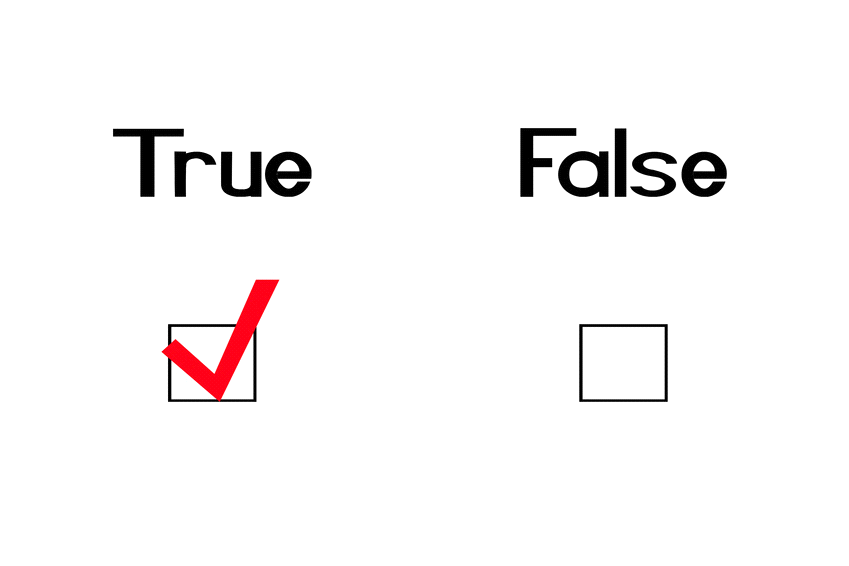
\includegraphics[width=0.4\textwidth]{pictures/TrueFalse.png}
\caption{True або False ?}
\label{TrueFalse} 
\end{center}
\end{figure}
\end{frame}

\begin{frame}
\frametitle{Логічні оператори}

\begin{table}
  \caption{Логічні вирази}
  \label{tab:}

  \begin{center}
    \begin{tabular}{|c|c|}
    \hline
      \textbf{Оператор} & \textbf{Значення} \\
    \hline  
      < & менше \\
    \hline
      >  & більше\\
    \hline
      <=  & менше або дорівнює \\
    \hline
      >=  & більше або дорівнює\\
    \hline
      ==  & дорівнює \\
    \hline
      !=  & не дорівнює \\
    \hline
    \end{tabular}
  \end{center}
\end{table}

\end{frame}

\begin{frame}
\frametitle{Логічні оператори}
\begin{table}
  \caption{Логічні оператори}
  \label{tab:}

  \begin{center}
    \begin{tabular}{|c|c|c|}
    \hline
      \textbf{Оператор} & \textbf{Значення} & \textbf{Пріоритет} \\
    \hline  
      or & або & 1 \\
    \hline
      and & та & 2 \\
    \hline
      not & ні & 3 \\
    \hline
    \end{tabular}
  \end{center}
\end{table}
\end{frame}

\subsection{Типове використання логічних операторів} 
\begin{frame}
\frametitle{Використання логічних операторів}
\begin{itemize}
  \item Перевірка на парність/непарність;
  \item Перевірка на потрапляння/непотрапляння в інтервал;
  \item Функція bool().
 \end{itemize}
\end{frame}

\subsection{Оператор розгалуження} 
\begin{frame}
\frametitle{Оператор if}
if - умовний оператор (оператор розгалуження).

% \begin{center}
\huge{if вираз:

~~~~операції}


\begin{flushleft}
\normalsize
Програма оцінює значення `вираз`, яке може дорівнювати True або False. Програма виконає операції тільки якщо вираз = True. Якщо вираз = False, цей шматок коду не буде виконуватись.
\end{flushleft}
% \end{center}
\end{frame}

\begin{frame}
\frametitle{Оператор if-else}
\Large{if вираз:

~~~~операції 1

else:

~~~~операції 2}


\begin{flushleft}
\normalsize
Операції 1 виконуються тільки якщо вираз істинний (дорівнює True). Якщо вираз дорівнює False, виконуються операції 2. Для розділення цих блоків використовуються відступи.
\end{flushleft}
% \end{center}
\end{frame}


\begin{frame}
\frametitle{Оператор if -elif-else}
\LARGE{if вираз 1:

~~~~операції 1

elif вираз 2:

~~~~операції 2

else:

~~~~операції 3}

\end{frame}

 \subsection{Використання умовного оператору} 
\begin{frame}
\frametitle{Знаходження мінімального}
\begin{figure}
\begin{center}
 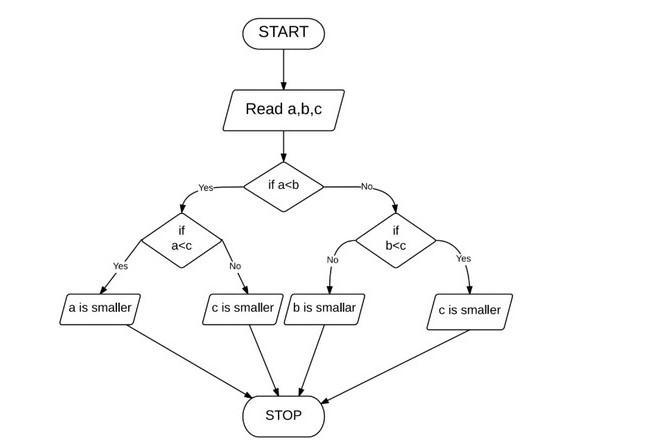
\includegraphics[width=0.4\textwidth]{pictures/find_min.jpg}
\caption{Алгоритм знаходження мінімального із трьох чисел}
\label{find_min} 
\end{center}
\end{figure}
\end{frame}

\begin{frame}
\frametitle{Тернарний умовний оператор}
У Python існує конструкція, яка за своєю дією аналогічна конструкції if-else, але є виразом. Вона називається тернарним оператором.

\Large{\texttt{значення\_1 if умова else значення\_2}}

Тернарний оператор повертає результат.
\end{frame}

\begin{frame}
\frametitle{Функції all та any}
Функція \texttt{all} повертає \texttt{True} якщо всі елементи переданого їй ітерованого об'єкту мають значення \texttt{True}.

Функція \texttt{any} повертає \texttt{True} якщо хоча б один елемент переданого їй ітерованого об'єкту має значення \texttt{True}.
\end{frame}

\subsection{Бітові операції} 
\begin{frame}
\frametitle{Операція НІ}
Бітова операція НІ виконує інверсію біт.

\begin{table}
  \caption{Бітова операція НІ}
  \label{tab:}

  \begin{center}
    \begin{tabular}{|c|c|}
    \hline
      \textbf{х} & \textbf{НІ} \\
    \hline
      0 & 1 \\
    \hline
      1 & 0 \\
    \hline
    \end{tabular}
  \end{center}
\end{table}

В Python бітова операція НІ позначається як $\sim x$.

\end{frame}

\begin{frame}
\frametitle{Операція І}

\begin{table}
  \caption{Бітова операція І: $x_1 \& x_2$}
  \label{tab:}

  \begin{center}
    \begin{tabular}{|c|c|c|}
    \hline
      \textbf{$x_1$} & \textbf{$x_2$} &  \textbf{І} \\
    \hline
      0 & 0 & 0 \\
    \hline
      0 & 1 & 0 \\
    \hline
      1 & 0 & 0 \\
    \hline
      1 & 1 & 1 \\
    \hline
    \end{tabular}
  \end{center}
\end{table}

Можна перевірити чи увімкнено або вимкнути відповідні біти.

\end{frame}

\begin{frame}
\frametitle{Операція АБО}

\begin{table}
  \caption{Бітова операція АБО: $x_1$ | $x_2$}
  \label{tab:}

  \begin{center}
    \begin{tabular}{|c|c|c|}
    \hline
      \textbf{$x_1$} & \textbf{$x_2$} &  \textbf{АБО} \\
    \hline
      0 & 0 & 0 \\
    \hline
      0 & 1 & 1 \\
    \hline
      1 & 0 & 1 \\
    \hline
      1 & 1 & 1 \\
    \hline
    \end{tabular}
  \end{center}
\end{table}

Можна перевірити чи увімкнено або вимкнути відповідні біти.

\end{frame}

\begin{frame}
\frametitle{Операція виключне АБО}

\begin{table}
  \caption{Бітова операція XOR: $x_1 \wedge x_2$}
  \label{tab:}

  \begin{center}
    \begin{tabular}{|c|c|c|}
    \hline
      \textbf{$x_1$} & \textbf{$x_2$} &  \textbf{XOR} \\
    \hline
      0 & 0 & 0 \\
    \hline
      0 & 1 & 1 \\
    \hline
      1 & 0 & 1 \\
    \hline
      1 & 1 & 0 \\
    \hline
    \end{tabular}
  \end{center}
\end{table}

За допомогою XOR можна перемикати біти числа.

\end{frame}

\begin{frame}
\frametitle{Зміщення біт}

\begin{itemize}
  \item $\gg$ - зміщення біт праворуч.
  \item  $\ll$  - зміщення біт ліворуч.

  \item $x = x \gg 1$ - еквівалентно цілочисленному діленню на два.

\end{itemize}


\end{frame}

% \section*{Лекція 6: Цикли}
 
 \subsection{Що таке цикл?} 
\begin{frame}
\frametitle{Цикл}
Цикли — оператори, які дозволяють повторювати код певну кількість разів.

\huge{цикл (умова):

~~~~операції
}

\normalsize Позначення:

\large{заголовок циклу:

~~~~тіло циклу
}


\end{frame}

\subsection{While} 
\begin{frame}
\frametitle{Цикл while}
Визначимо суму чисел від 1 до N.

s = 0

i = 1 

N = 1000

while i <= N:

~~~~s += i

~~~~i += 1

Одноразове виконання тіла цикла називається ітерацією цикла.

\end{frame}

\begin{frame}
\frametitle{Корисні оператори для циклу while}
\begin{itemize}
  \item break - дострокове завершення циклу.
  \item continue - пропуск однієї ітерації циклу.
  \item В блоці else йдуть команди, що виконуються після штатного завершення циклу.
\end{itemize}
\end{frame}

 \subsection{For} 
\begin{frame}
\frametitle{Цикл for}
\huge{for змінна in ітератор:

~~~~операції
}

\normalsize 
У циклі for вказується змінна і низка значень, на які буде послатися змінна в різних ітераціях. Значення можуть бути задані списком, кортежем, рядком тощо. Значення, на які посилається змінна в циклі \underline{не змінюються} (для такої зміни слід звертатися до елементів за індексом).

\end{frame}

\begin{frame}
\frametitle{Функція range}
Функція \texttt{range()} генерує ряд чисел у межах заданого діапазону. Можна визначити початок та кінець цього ряду, а також якою буде різниця між двома числами.

\begin{itemize}
  \item \texttt{range(stop)}
  \item \texttt{range(start, stop)}
  \item \texttt{range(start, stop, step)}
\end{itemize}
\end{frame}

\begin{frame}
\frametitle{Приклади застосування циклу for}
\begin{enumerate}
  \item 
  Розрахунок факторіалу натурального числа n:

\begin{center}
n! = 1*2*3*...*(n-1)*n
\end{center}
\item 
Відобразити ялинку:

*

**

***

****

\item 
Задано список із цілих чисел. Треба замінити кожне двозначне число на нуль.
\end{enumerate}
\end{frame}

\begin{frame}
\frametitle{Функція enumerate}
Іноді, при переборі об'єктів у циклі for, потрібно як отримати сам об'єкт, а й його порядковий номер. Це можна зробити за допомогою ітератора enumerate:

\huge{for i, el in enumerate(lst):

~~~~операції}
\end{frame}

\subsection{Ітератори} 
\begin{frame}
\frametitle{Що таке ітератор?}
Об'єкт, що ітерується (iterable) - це об'єкт, який може повертати елементи по одному, з нього можна одержати ітератор.

Приклади об'єктів, що ітеруються:

\begin{itemize}
  \item всі послідовності: список, рядок, кортеж
  \item словники
  \item файли 
\end{itemize}
    
Ітератор використовується для одноразового перебору елементів об'єкту.
\end{frame}

\begin{frame}
\frametitle{Функції iter та next}
Функція \texttt{iter()} повертає ітератор і створює об'єкт, який може перебиратися по одному елементу за раз.

Щоб отримати наступне значення з ітератора, використовується функцію \texttt{next()}. Не можна використовувати \texttt{next()} зі списком чи кортежем, але можна зробити список, кортеж або рядок ітератором (функцією \texttt{iter()}), а потім використати \texttt{next()}.

Якщо ітерований об'єкт пройдено до кінця, то застосування до нього функції \texttt{next()} призводе до помилки StopIteration.
\end{frame}

\subsection{Вкладені цикли} 
\begin{frame}
\frametitle{Вкладені цикли}
Вкладені цикли використовуються для роботи із вкладеними списками або із списками ітерованих об'єктів.

\huge{
for i in iterator\_1:

~~~~for j in iterator\_2:

~~~~~~~~operations
}
\end{frame}

\begin{frame}
\frametitle{Застосування вкладених циклів}
Для транспонування вкладеного списку A  використовується програма:

% \texttt{
for i in range(N):

~~~~for j in range(i+1, N):

~~~~~~~~A[i][j], A[j][i] = A[j][i], A[i][j]
% }
\end{frame}

\begin{frame}
\frametitle{Застосування вкладених циклів}
\begin{figure}
\begin{center}
 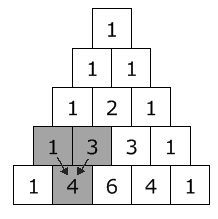
\includegraphics[width=0.4\textwidth]{pictures/pascal.png}
\caption{Трикутник Паскаля}
\label{pascal} 
\end{center}
\end{figure}
\end{frame}

% \section{Лекція 7: Словники та кортежі}
 
 \subsection{Що таке словник?} 
\begin{frame}
% \frametitle{Логічні висновки}
Словник – невпорядкована структура даних, що дозволяє зберігати пари «ключ – значення». Їх іноді ще називають асоціативними масивами чи хеш-таблицями.

\begin{figure}
\begin{center}
 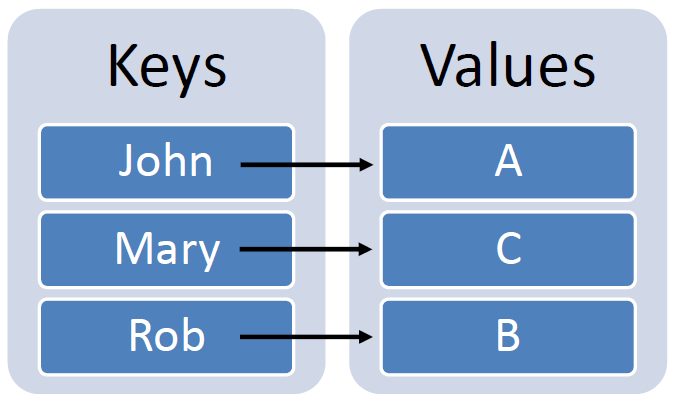
\includegraphics[width=0.4\textwidth]{pictures/dict.png}
\caption{Словник}
\label{dict} 
\end{center}
\end{figure}

\end{frame}

\begin{frame}
% \frametitle{Логічні висновки}

\begin{itemize}
  \item 
  Приклад словника d:

 d = \{ключ\_1: значення\_1,
 
  ключ\_2: значення\_2, ... 

ключ\_N: значення\_N\}
\item Доступ до значення словника: d[ключ].

\item
Створювати словники можна за допомогою конструкції:

d = dict(ключ\_1 = значення\_1, ...

 ключ\_N = значення\_N)
 
 \item Визначення пустого словника d = \{\} або d = dict()
\end{itemize}

\end{frame}

\begin{frame}
% \frametitle{Логічні висновки}
Ключом в словнику можуть бути тільки дані незмінного типу. Значеннями можуть бути дані будь-якого типу.

\begin{itemize}
  \item Для визначення числа елементів в словнику використовується функція \texttt{len}.
  
  \item Для видалення ключа \texttt{key} та його значення із словника \texttt{d} використовується команда \texttt{del d[key]}.
  \item Для перевірки, що ключ \texttt{key} присутній в словнику \texttt{d}, використовується команда \texttt{key in d}.
  \item Для перевірки, що ключ \texttt{key} відсутній в словнику \texttt{d}, використовується команда \texttt{key not in d}.
\end{itemize}
\end{frame}

\subsection{Методи словника d} 
\begin{frame}
    \begin{itemize}
        \item<1-> \texttt{d = dict.fromkeys(lst[, val])} - створює словник d, ключами якого є елементи списку lst, необов'язковий аргумент val - значення за замовчуванням;
        \item<2-> \texttt{d.clear()} - очищує словник d;
        \item<3-> \texttt{d.copy()} - створює копію словника d (інший варіант створення копії словника - функція \texttt{dict(d)} );
        \item<4-> \texttt{d.get(key)} - отримати значення по ключу key зі словника d (на відміну від \texttt{d[key]}, при звертанні до неіснуючого ключа повертає \texttt{None} або другий параметр методу \texttt{get});
    \end{itemize}
\end{frame}

\begin{frame}
    \begin{itemize}
        \item<1-> \texttt{d.setdefaults(key[, val])} - якщо ключ key є в словнику d, то повертає значення за цим ключом, інакше повертає None (або необов'язковий параметр val) та додає до словника значення None (або необов'язковий параметр val) за ключом key;
        \item<2-> \texttt{d.pop(key[, val])} - видаляє значення за ключем key зі словника d та повертає це значення, для неіснуючого ключа key повертає помилку або необов'язковий параметр val;
        \item<3-> \texttt{d.popitem()} - видаляє та повертає значення за випадковим ключем зі словника d;
    \end{itemize}
\end{frame}

\begin{frame}
    \begin{itemize}
        \item<1-> \texttt{d.keys()} - повертає список ключів словника d;
        \item<1-> \texttt{d.values()} - повертає список значень словника d;
        \item<1-> \texttt{d.items()} - повертає список кортежів із ключів та значень словника d;
        \item<2-> \texttt{d.update(d1)} - оновлює словник d значеннями зі словника d1;
        \item<3-> \texttt{d = \{**d1, **d2\}} - поєднання словників d1 та d2 у словник d.
    \end{itemize}
\end{frame}


 \subsection{Що таке кортеж?} 
\begin{frame}
% \frametitle{Логічні висновки}
Кортеж (turple) – впорядкована, але незмінна колекція довільних даних.

\begin{figure}
\begin{center}
 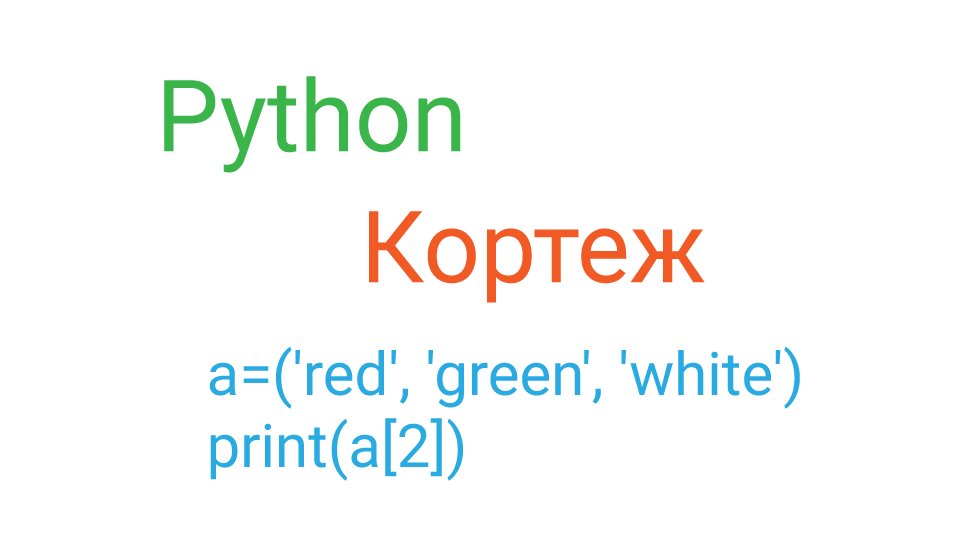
\includegraphics[width=0.4\textwidth]{pictures/turple.png}
\caption{Кортеж}
\label{turple} 
\end{center}
\end{figure}

\end{frame}

\begin{frame}
% \frametitle{Логічні висновки}
Для створення кортежу треба вказувати кому, дужки не є обов'язковими. Варіанти створення кортежу:

\begin{itemize}
  \item a = (1, 2, 3)
  \item a = 1, 2, 3
  \item a = (1,)
  \item a = 1,
\end{itemize}

Розпакування кортежу в змінні:

x, y = (1, 2)
\end{frame}

 \subsection{Функції для роботи з кортежами} 
\begin{frame}
% \frametitle{Логічні висновки}
\begin{itemize}
  \item \texttt{len(t)} - знаходження довжини  кортежу \texttt{t};
  \item \texttt{t[i]} - звертання до \texttt{i}-го елементу  кортежу \texttt{t};
  \item \texttt{t[:i:j]} - зрізи працюють так само як і для списків, лише операція \texttt{t[:]} не створює копію, а посилається на той самий кортеж \texttt{t};
  \item в кортежах не можна змінювати дані \texttt{t[i] = j} - помилка;
  \item кортежі можна використовувати як ключі словників;
\end{itemize}

\end{frame}

\begin{frame}
% \frametitle{Логічні висновки}
\begin{itemize}
  \item \texttt{t = ()} або \texttt{t = turple()} - створення пустого кортежу;
  \item \texttt{t + (1,)} - додавання елементу до кортежу;
  \item \texttt{(1,)*n} - дублювання елементів кортежу \texttt{n} разів;
  \item \texttt{turple(it)} - створює кортеж із елементів будь-якого ітерованого об'єкту \texttt{it};
  \item \texttt{val in t} - перевіряє чи ходить елемент \texttt{val} в кортеж \texttt{t}.
\end{itemize}

\end{frame}

\subsection{Методи кортежу t} 
\begin{frame}
    \begin{itemize}
        \item<1-> \texttt{t.count(val)} - повертає число знайдених елементів із значенням \texttt{val};
        \item<2-> \texttt{t.index(val, start, stop)} - повертає індекс першого знайденого елементу із значенням \texttt{val}, \texttt{start} та \texttt{stop} індекси початку та кінця пошуку (необов'язкові параметри).
    \end{itemize}
\end{frame}

 \subsection{Що таке множина?} 
\begin{frame}
% \frametitle{Логічні висновки}
Множина (set) – невпорядкована колекція унікальних елементів.

\begin{figure}
\begin{center}
 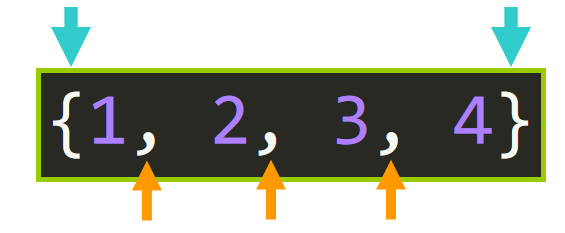
\includegraphics[width=0.4\textwidth]{pictures/set.png}
\caption{Множина}
\label{set} 
\end{center}
\end{figure}

\end{frame}

\begin{frame}
% \frametitle{Логічні висновки}
\begin{itemize}
  \item \texttt{a = \{1, 2, 3, "hello"\}} - множина;
  \item елементи множини - незмінні типи даних (числа, булеві значення, рядки, кортежі);
  \item не можуть бути елементами множин - списки, словники, інші множини;
  \item \texttt{s = set()} - пуста множина;
  \item \texttt{s = set(it)} - створює множину із унікальних елементів ітерованого об'єкту \texttt{it};
  \item звернутися до елементу множини за індексом неможливо;
  \item множина - ітерований об'єкт.
\end{itemize}

\end{frame}

 \subsection{Функції для роботи з множиною} 
\begin{frame}
% \frametitle{Логічні висновки}
\begin{itemize}
  \item \texttt{len(s)} - повертає кількіть елементів у множині \texttt{s};
  \item \texttt{val in s} - перевірка чи присутній елемент \texttt{val} у множині \texttt{s};
  \item \texttt{s.add(val)} - додає елемент \texttt{val} у множину \texttt{s};
  \item \texttt{s.update(it)} - додає елементи ітерованого об'єкту \texttt{it} у множину \texttt{s};
\end{itemize}
\end{frame}

\begin{frame}
% \frametitle{Логічні висновки}
\begin{itemize}

  \item \texttt{s.discard(val)} - видаляє елемент \texttt{val} із множини \texttt{s} (якщо елемент \texttt{val} відсутній у множині \texttt{s} - нічого не повертає);
  \item \texttt{s.remove(val)} - видаляє елемент \texttt{val} із множини \texttt{s} (якщо елемент \texttt{val} відсутній у множині \texttt{s} - повертає помилку);
  \item \texttt{s.pop()} - повертає та видаляє довільний елемент із множини \texttt{s} ;
  \item \texttt{s.clear()} - видаляє всі елементи із множини \texttt{s}.
\end{itemize}

\end{frame}

 \subsection{Операції над множинами} 
\begin{frame}
% \frametitle{Логічні висновки}
\begin{itemize}
  \item \texttt{s1 \& s2} (або \texttt{s1.intersection(s2)}) - повертає множину, що є перетином множин \texttt{s1} та \texttt{s2};
  \item \texttt{s1 = s1 \& s2} (або \texttt{s1 \&= s2} або \texttt{s1.intersection\_update(s2)}) - записує до множини \texttt{s1} множину, що є перетином множин \texttt{s1} та \texttt{s2};
  \end{itemize}
 \begin{figure}
\begin{center}
 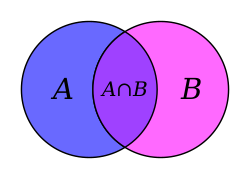
\includegraphics[width=0.25\textwidth]{pictures/intersection.png}
\caption{Перетин множин}
\label{intersection} 
\end{center}
\end{figure} 
  
\end{frame}

\begin{frame}
% \frametitle{Логічні висновки}
\begin{itemize}
    \item \texttt{s1 | s2} (або \texttt{s1.union(s2)}) - повертає множину, що є об'єднанням множин \texttt{s1} та \texttt{s2};
  \item \texttt{s1 = s1 | s2} (або \texttt{s1 |= s2} ) - записує до множини \texttt{s1} множину, що є об'єднанням множин \texttt{s1} та \texttt{s2};
\end{itemize}
 \begin{figure}
\begin{center}
 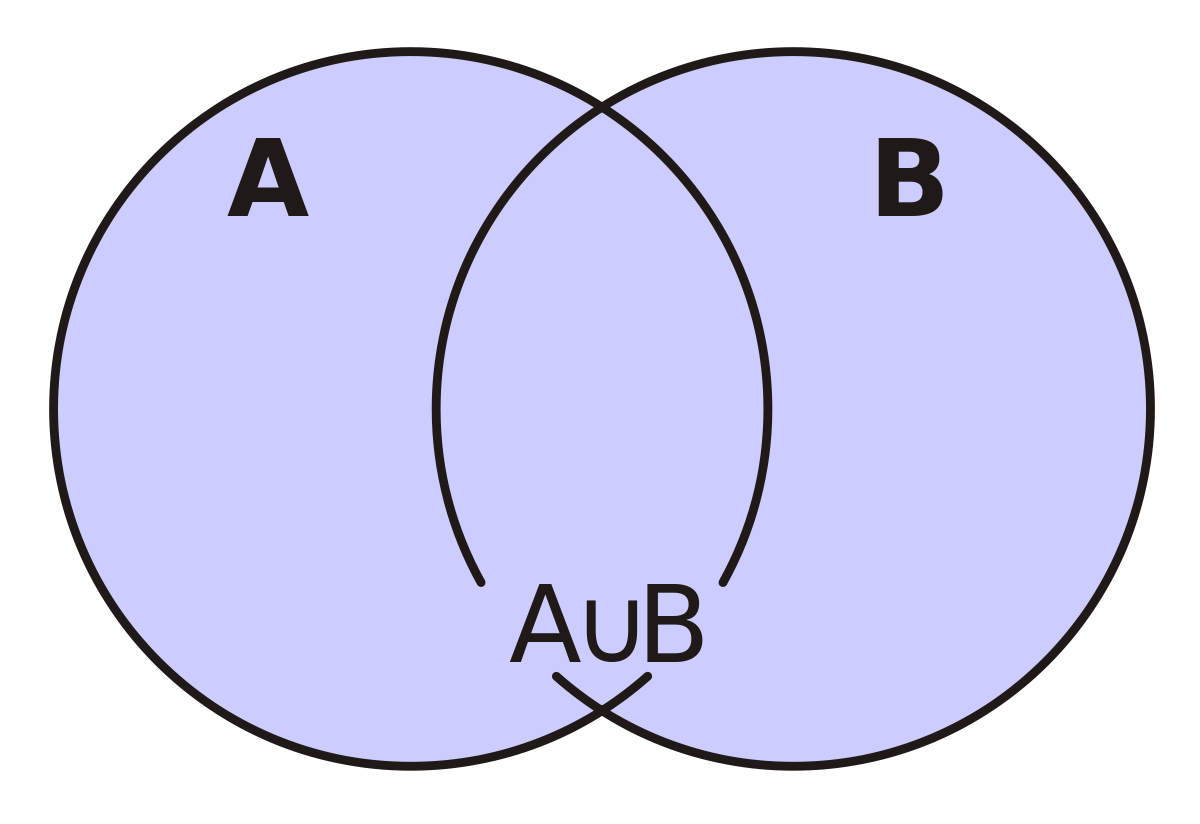
\includegraphics[width=0.25\textwidth]{pictures/union.png}
\caption{Об'єднання множин}
\label{union} 
\end{center}
\end{figure} 
\end{frame}

\begin{frame}
% \frametitle{Логічні висновки}
\begin{itemize}
    \item \texttt{s1 - s2} - повертає множину, що є різницею множин \texttt{s1} та \texttt{s2};
  \item \texttt{s1 -= s2} - записує до множини \texttt{s1} множину, що є різницею множин \texttt{s1} та \texttt{s2};
\end{itemize}
 \begin{figure}
\begin{center}
 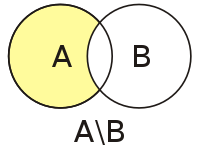
\includegraphics[width=0.25\textwidth]{pictures/subtract.png}
\caption{Різниця множин}
\label{subtract} 
\end{center}
\end{figure} 
\end{frame}

\begin{frame}
% \frametitle{Логічні висновки}
\begin{itemize}
    \item \texttt{s1 $\hat{}$ s2} - повертає множину, що є симетричною різницею множин \texttt{s1} та \texttt{s2};
%   \item \texttt{s1 -= s2} - записує до множини \texttt{s1} множину, що є різницею множин \texttt{s1} та \texttt{s2};
\end{itemize}
 \begin{figure}
\begin{center}
 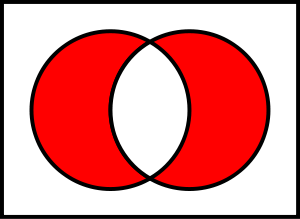
\includegraphics[width=0.25\textwidth]{pictures/xor.png}
\caption{Симетрична різниця множин}
\label{xor} 
\end{center}
\end{figure} 
\end{frame}

\begin{frame}
\frametitle{Порівняння множин}
Множини є рівними, якщо їх довжина та значення елементів співпадають. Множина \texttt{s1} входе в множину \texttt{s2}, якщо всі елементи множини \texttt{s1} містяться в більшій множині \texttt{s2}.
\begin{itemize}
    \item \texttt{s1 == s2} (\texttt{s1 != s2}) - перевірка на рівність (нерівність) множин;
    \item \texttt{s1 < s2} - перевірка, що множина \texttt{s1}  входе у множину \texttt{s2};
    \item \texttt{s1 <= s2} - перевірка, що множина \texttt{s1}  входе у множину \texttt{s2}, або вони є рівними.
\end{itemize}
\end{frame}

% \section{Лекція 8: Генератори}
 
 \subsection{Що таке генератор?} 
\begin{frame}
% \frametitle{Логічні висновки}
У Python є спеціальна синтаксична конструкція, яка дозволяє за певними правилами створювати заповнені списки. Такі конструкції називають генераторами списків (list comprehension). Їх зручність полягає у більш короткому запису програмного коду, ніж якби створювався список звичайним способом.

\LARGE{[правило for змінна in ітератор]}

\normalsize або

\LARGE{[правило for змінна in ітератор if умова]}

\normalsize Наприклад:

[i**2 for i in range(N)]

\end{frame}

\begin{frame}
% \frametitle{Логічні висновки}
Генератори списків можуть бути вкладені.

\LARGE{[правило

 for змінна\_1 in ітератор\_1 if умова\_1
 
 ...
 
 for змінна\_N in ітератор\_N if умова\_N]}

\normalsize Така конструкція працює так само як низка вкладених циклів \texttt{for}.

\end{frame}

\begin{frame}
% \frametitle{Логічні висновки}
В якості \textit{правила} в генераторі списку можна використовувати ще один генератор списку.

\Large{[[ правило for змінна\_1 in ітератор\_1 if умова\_1]

 for змінна\_2 in ітератор\_2 if умова\_2]}

\end{frame}

\begin{frame}
% \frametitle{Логічні висновки}
Вкладений генератор списку можна використовувати для транспонування прямокутної матриці A:

\vspace{1cm}

\large{[[ row[i] for row in A] for i in range(len(A[0]))]}

\end{frame}

\begin{frame}
% \frametitle{Логічні висновки}
Генератор списку може використовуватися як ітератор для генератору списку.

\vspace{1cm}

\LARGE{[правило\_2 for змінна\_2 in 

[правило\_1 for змінна\_1 in ітератор]]}

\vspace{1cm}

\normalsize Такий генератор працює як вкладена фукнція.

\end{frame}

 \subsection{Генератор множин} 
\begin{frame}
% \frametitle{Логічні висновки}
Аналогічно до генераторів списків можна побудувати генератор множин.

\LARGE{\{правило for змінна in ітератор\}}

\normalsize або

\LARGE{\{правило for змінна in ітератор if умова\}}

\end{frame}

 \subsection{Генератор словника} 
\begin{frame}
% \frametitle{Логічні висновки}
Словник можна отримати за допомогою генератора, аналогічного до генератору списку або множини.

\Large{\{ключ: значення for змінна in ітератор\}}

\normalsize або

\Large{\{ключ: значення for змінна in ітератор if умова\}}

\end{frame}

\begin{frame}
% \frametitle{Логічні висновки}
Для генераторів списків, множин та словників працює внутрішній генератор, що створює елементи цих об'єктів. Щоб створити такий генератор використовується синтаксис:
\Large{(правило for змінна in ітератор)}

\normalsize або

\Large{(правило for змінна in ітератор if умова)}

\normalsize Генератор можна перебирати тільки один раз. Функції list, set, tuple, sum, max, min можуть приймати як аргумент генератор. Генератори не зберігають в пам'яті всі значення, а створюють їх за необхідності.


\end{frame}

\subsection{Функція-генератор} 
\begin{frame}
% \frametitle{Логічні висновки}
Щоб перетворити функцію в функцію-генератор слід замість оператору \texttt{return} використовувати оператор \texttt{yield}.
\end{frame}

\begin{frame}
% \frametitle{Логічні висновки}
Фукнція \texttt{map} застосовує функцію \texttt{func} до кожного елементу ітератору \texttt{it}, як результат отримується генератор \texttt{gen}: \texttt{gen = map(func, it)}. 

Функція map еквівалентна генератору:

\texttt{(func(x) for x in it)}

Всередині фукнції \texttt{map} можна використовувати \texttt{lambda}-функцію. 
\end{frame}

\begin{frame}
% \frametitle{Логічні висновки}
Фукнція \texttt{filter} слугує для фільтрації елементів ітерованого об'єкту.

\texttt{filter(func, it)}

Якщо функція \texttt{func} повертає значення \texttt{True}(\texttt{False}) для поточного значення ітерованого об'єкту, то це значення повертається (не повертається).

Всередині фукнції \texttt{filter} можна використовувати \texttt{lambda}-функцію. Як ітерований об'єкт \texttt{it} всередині функції \texttt{filter}  можна використовувати результат роботи іншої функції \texttt{filter}.
\end{frame}

\begin{frame}
% \frametitle{Логічні висновки}
Фукнція \texttt{zip(it\_1[, it\_2 , it\_3])} для вказаних ітерованих об'єктів здійснює відповідних перебір і продовжує роботу доки не дійде до кінця самої короткої колекції. В результаті отримуємо ітератор кортежів.

\end{frame}

% \section*{Лекція 9: Основи використання функцій в Python}
 
 \subsection{Що таке функція?} 
\begin{frame}
\frametitle{Функція}
Функція — частина програми, яка реалізує певний алгоритм і дозволяє звернення до неї з різних частин програми.
\begin{figure}
  \begin{center}
    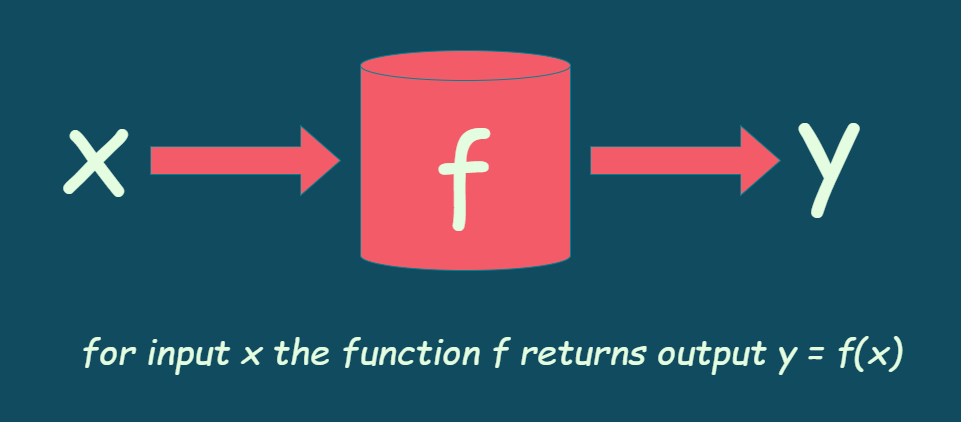
\includegraphics[width=\textwidth,height=0.4\textheight]{pictures/function.png}
  \caption{Функція}
\label{function}
  \end{center}
\end{figure}
\end{frame}

\begin{frame}
\frametitle{Функція print}
Приклад функції — \texttt{print}. При цьому \texttt{print} - посилання на об'єкт функцію (і воно може бути змінено, наприклад: \texttt{f = print}), а конструкція \texttt{print()} дозволяє запустити функцію на виконання.

\begin{center}
\large{DRY - Don't Repeat Yourself}
\end{center}

\normalsize Частини програми, що повторюються, слід розмістити в об'єкт функцію, а потім їх викликати в потрібних місцях.
\end{frame}

\begin{frame}
\frametitle{Синтаксис функції}
Синтаксис створення власної функції в Python:

\Large{def назва(список аргументів):

~~~~оператор 1

~~~~... 

~~~~оператор N }

\vspace{0.5cm}
\normalsize Аргумент всередині функції називається \textit{параметр}, а значення, що передається функції, підчас її виклику - \textit{аргумент}.
\end{frame}

 \subsection{Властивості функцій} 
\begin{frame}
\frametitle{Оператор return}
Після \texttt{return} вказується значення, яке повертає функція.

\Large{def назва(список аргументів):

~~~~оператор 1

~~~~... 

~~~~оператор N

~~~~return значення }

\normalsize Щоб повернути декілька змінних використовується кортеж.

\end{frame}

\begin{frame}
\frametitle{Властивості функцій}
\begin{itemize}
  \item Всередині функцій можна викликати інші функції.
  \item Функції можна визначати всередині різних конструкції мови програмування (умовні оператори, цикли, інші функції тощо).

\end{itemize}

\end{frame}

\begin{frame}
\frametitle{Приклад застосування функцій}
Найбільший спільний дільник (НСД) чисел — найбільше натуральне число, на яке ці числа діляться без остачі. 

Алгоритм Євкліда для знаходження НСД чисел a та b:

\texttt{доки а != b} 

~~~~\texttt{знаходимо найбільше серед а та b}


~~~~\texttt{зменшуємо більше на величину меншого}

\texttt{виводимо а (або b)}

\end{frame}

\begin{frame}
\frametitle{Приклад застосування функцій}
Найбільший спільний дільник (НСД) чисел — найбільше натуральне число, на яке ці числа діляться без остачі. 


Швидкий алгоритм Євкліда:

\texttt{доки менше число більше 0}

~~~~\texttt{більше число = залишок від ділення на менше} 

\texttt{виводимо більше число}
\end{frame}

\subsection{Параметри функцій} 
\begin{frame}
\frametitle{Позиційні та іменовані аргументи}
Якщо є функія \texttt{def func(a, b, c) ...} , то

\begin{itemize}
  \item При виклику функції позиції параметрів відповідають позиціям аргументів (позиційний запис аргументів) \texttt{func(1, 2, 3)}.
  \item При використанні іменованих аргументів можна передати параметрам функції значення із інших позицій аргументів \texttt{func(b=1, c=2, a=3)} або \texttt{func(1, c=2, =3)}.
\end{itemize}

\end{frame}


\begin{frame}
\frametitle{Фактичні та формальні параметри}
Якщо є функія \texttt{def func(a, b, c=1, d=2) ...} , то
\begin{itemize}
  \item \texttt{a} та \texttt{b} - фактичні параметри;
  \item \texttt{c} та \texttt{d} - формальні параметри;
  \item \texttt{1}  та \texttt{2} - значення за замовчуванням. 
\end{itemize}

Формальні параметри при виклику функції можна не вказувати, в цьому випадку використовуються значення за замовчуванням. Щоб задати значення формальних параметрів можна викликати функцію як \texttt{func(3, 4, c=2, d=1)} або як \texttt{func(3, 4, 2, 1)}.


\end{frame}


\begin{frame}
\frametitle{Функції з довільним числом аргументів}
\begin{itemize}
  \item \texttt{def func(*args) ...} - довільне число формальних аргументів (\texttt{args} - кортеж із довільного числа параметрів. 
  \item \texttt{def func(*args, par1=1, par2=2) ...}  - довільне число формальних аргументів та фактичні аргументи.
  \item \texttt{def func(*args, **kwargs) ...} - довільне число формальних аргументів та фактичних аргументів.
\end{itemize}
\end{frame}

\begin{frame}
\frametitle{Функції з довільним числом аргументів}
\begin{itemize}
  \item \texttt{func(*args, p1=1, **kwargs) ...} - довільне число формальних і фактичних та фактичний аргумент.
   \item \texttt{def func(arg1, *args, p1=1, **kwargs) ...}  - довільне число формальних та фактичних, один формальний та конкретний фактичний аргумент.
\end{itemize}

\end{frame}

\subsection{Упаковка та розпаковка колекцій} 
\begin{frame}
\frametitle{Упаковка колекцій}
\begin{itemize}
  \item Упаковка \texttt{x, *y = (1, 2, 3, 4)} або \texttt{*x, y = (1, 2, 3, 4)}
  \item Упаковка \texttt{x, *y = [1, "a", True, 4]} або \texttt{*x, y = "Hello!"}
  \item \texttt{*x = 1, 2, 3} - помилка
\end{itemize}

\end{frame}

\begin{frame}
\frametitle{Розпаковка колекцій}
\begin{itemize}
  \item Розпаковка списку \texttt{a = [1, 2, 3]} в кортеж \texttt{(*a,)}
  \item Розпаковка кортежу \texttt{a = -5, 5} в оператор \texttt{range(*a)}
  \item Щоб отримати список \texttt{*range(*a)}
  \item Розпаковка словника в словник \texttt{**d}
  \item Об'єднання словників \texttt{**d, **d1} 
\end{itemize}

\end{frame}

% \section{Лекція 10: Функції}
 
 \subsection{Рекурсивні функції} 
\begin{frame}
% \frametitle{Логічні висновки}
Рекурсивна функція — функція, що викликає саму себе. При цьому функція розміщується в стек виклику функції. Кількість внутрішніх викликів функції називається глибиною рекурсії.
\begin{figure}
  \begin{center}
    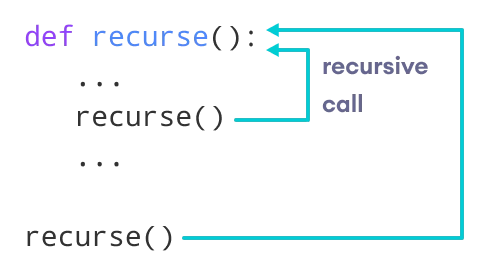
\includegraphics[width=0.5\textwidth,height=0.5\textheight]{pictures/recursion.png}
  \caption{Рекурсивна функція}
\label{function}
  \end{center}
\end{figure}
\end{frame}

\begin{frame}
% \frametitle{Логічні висновки}
Приклад рекурсивної функції:

\vspace{1cm}

\texttt{def recursive(value):}

\texttt{~~~~print(value)}

\texttt{~~~~if value < 4:}

\texttt{~~~~~~~~recursive(value)}

\texttt{~~~~print(value)}

\end{frame}

\subsection{Lambda-функції} 
\begin{frame}
% \frametitle{Логічні висновки}
Lambda-функція — анонімна функція.

\Large{\texttt{lambda param\_1, param\_2, ... : команда}}

\normalsize
\begin{itemize}
  \item lambda-функція автоматично повертає результат свого виконання (оператор return не потрібен);
  \item lambda-функція зазвичай присвоюється якійсь змінній; 
  \item lambda-функція може бути елементом будь-якої конструкції мови Python;
  \item всередині lambda-функції не можна виконувати присвоювання.
\end{itemize}

\end{frame}

\begin{frame}
% \frametitle{Логічні висновки}
Приклад використання lambda-функції:

\texttt{def get\_filter(a, filter=None):}

\texttt{~~~~ if filter is None:}

\texttt{~~~~~~~~return a}

\texttt{~~~~res = []}

\texttt{~~~~for filter in a:}

\texttt{~~~~~~~~if filter(x):}

\texttt{~~~~~~~~~~~~res.append(x)}

\texttt{~~~~return res}

\vspace*{0.8cm}

\texttt{print(get\_filter(a))}

\texttt{print(get\_filter(a, filter=lambda x: x \% 2 == 0))}
\end{frame}

\subsection{Простір імен} 
\begin{frame}
% \frametitle{Логічні висновки}
Локальний простір імен: простір імен містить локальні імена всередині функції. Цей простір імен створюється під час виклику функції і продовжується, поки функція не повернеться.

Глобальний простір імен: це простір імен, який включає імена різних імпортованих модулів, які ви використовуєте в проекті. Він створюється, коли модуль включений у проект, і існує до завершення виконання програми.

\end{frame}

\subsection{Область видимості} 
\begin{frame}
% \frametitle{Логічні висновки}
Локальна область видимості є внутрішньою областю, яка містить список локальних імен, доступних у поточній функції.

Глобальна область  видимості - область всіх функцій, що закривають. 

Пошук імені починається з найближчої області, що охоплює, і переміщається назовні.

Щоб всередині функції змінити глобальну змінну \texttt{var} використовується команда \texttt{global var}.

Щоб всередині функції працювати зі змінною \texttt{var} із зовнішнього (локального) простору імен використовується команда \texttt{nonlocal var}.

\end{frame}

\section{Лекція 11: Робота з файлами}
 
 \subsection{Функція open} 
\begin{frame}
% \frametitle{Логічні висновки}
Для того, щоб отримати доступ до файлу використовується функція \texttt{open}:

\texttt{f = open(file[, mode='r', encoding=None, ...])}

\begin{itemize}
  \item \texttt{file} - шлях до файлу;
  \item \texttt{mode} - режим доступу до файлу (читання/запис);
  \item \texttt{encoding} - кодування файлу.
\end{itemize}

\texttt{f.read()} - читає весь вміст файлу \texttt{f}. 
\end{frame}

\begin{frame}
% % \frametitle{Логічні висновки}
\texttt{f.read(4)} - читає перші 4 символи файлу \texttt{f} (читання розпочинається з місця, на яке вказує файлова позиція). Файлова позиція вказується в байтах.

Для встановлення файлової позиції в положення \texttt{offset} використовується функція \texttt{f.seek(offset[, from\_what])}.

Метод \texttt{f.tell()} повертає поточну файлову позицію.

Метод \texttt{f.readline()} читає рядок із файлу.
%
\texttt{f} сприймається як ітерований об'єкт і при ітерації повертає новий прочитаний рядок із файлу.

Метод \texttt{f.readlines()} читає вміст файлу та повертає список із рядків файлу.

\texttt{f.close()} закриває файл.
\end{frame}

\begin{frame}
% % \frametitle{Логічні висновки}
Якщо файл не знайдено виникає помилка \texttt{FileNotFoundError}. Для обробки таких та подібних виключень використовується конструкція:

\texttt{try:}

\texttt{~~~~operators\_1}

\texttt{except [виключення]:}

\texttt{~~~~operators\_2}

\texttt{finally:}

\texttt{~~~~operators\_3}

Блок \texttt{finally} виконується в будь-якому випадку якщо трапилось виключення, або якщо не трапилось.

\end{frame}

\begin{frame}
% % \frametitle{Логічні висновки}
Уникнути зупинки програми у випадку помилки при роботі з файлом можна за допомогою менеджера контексту:

\texttt{with open(file\_path) as file:}

\texttt{~~~~operators}

Виконання блоку \texttt{with} завжди завершується закриттям файлу.

\end{frame}

\begin{frame}
% % \frametitle{Логічні висновки}
\begin{itemize}
  \item \texttt{open(file\_path)} або \texttt{open(file\_path,"r")} - відкриття файлу для читання.
  \item \texttt{open(file\_path,"w")} - відкриття файлу для запису.
  \item \texttt{open(file\_path,"a")} - відкриття файлу для дозапису.
  \item \texttt{open(file\_path,"a+")} - відкриття файлу для дозапису та читання.
\end{itemize}
Для запису рядка \texttt{string} до файлу використовується метод \texttt{file.write(string)}. Метод \texttt{file.writelines(lst)} записує відразу декілька рядків до файлу, кожен рядок відповідає елементу списка \texttt{lst}.
\end{frame}

\begin{frame}
% % \frametitle{Логічні висновки}
Можна працювати з бінарними файлами.
\begin{itemize}
  \item \texttt{open(file\_path,"rb")} - відкриття бінарного файлу для читання.
  \item \texttt{open(file\_path,"wb")} - відкриття бінарного файлу для запису.
\end{itemize}
Для роботи з бінарними файлами використовується модуль \texttt{pickle}: \texttt{import pickle}.
Для запису до файлу \texttt{file} даних \texttt{data} у бінарному вигляді використовується метод \texttt{pickle.dump(data, file)}. Для зчитування даних із бінарного файлу \texttt{file} використовується метод \texttt{pickle.load(file)}.
\end{frame}

% \section*{Лекція 13: Модулі та імпорт}
 
 \subsection{Імпорт модулів} 
\begin{frame}
\frametitle{Стандартні модулі Python}
\begin{figure}
  \begin{center}
    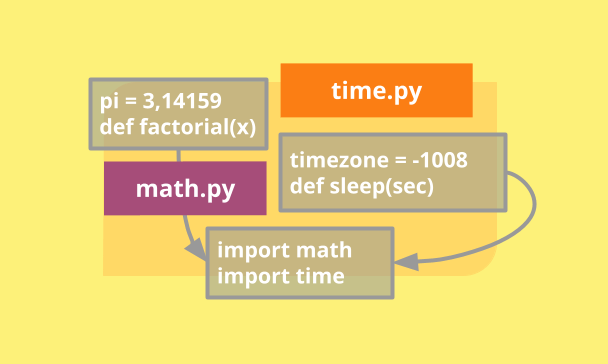
\includegraphics[width=0.4\textwidth,height=0.35\textheight]{pictures/import.png}
  \caption{Модулі Python}
\label{function}
  \end{center}
\end{figure}


Python має велику кількість стандартних \href{https://docs.python.org/3/library/}{бібліотек}.

\end{frame}

\begin{frame}
\frametitle{Команди для роботи з модулями}
\begin{itemize}
  \item<1-> \texttt{import module} додає до глобального простору простор імен визначені в модулі \texttt{module} змінні, функції, класи:
  \begin{center}
  \texttt{module.fun()}
  \end{center} 
  \item<2-> \texttt{import module as mod} вказує псевдонім \texttt{mod} модуля \texttt{module}:
  \begin{center}
  \texttt{mod.fun()}
  \end{center} 

\end{itemize}

\end{frame}

\begin{frame}
\frametitle{Команди для роботи з модулями}
\begin{itemize}
  \item<1-> \texttt{from module import *} - імпортує весь вміст модуля \texttt{module}.
  \item<2-> \texttt{from module import fun} - імпортує функцію \texttt{fun} із модуля \texttt{module}:
   \begin{center}
  \texttt{fun()}
  \end{center} 
  \item<3-> \texttt{from module import fun as function} - вибірковий імпорт функції \texttt{fun} з псевдонімом \texttt{function} із модуля \texttt{module}:
  \begin{center}
  \texttt{function()}
  \end{center}
\end{itemize}
\end{frame}

\begin{frame}
\frametitle{Пакети}
Пакет (package) - спеціальним чином організований підкаталог з низкою модулів, що зазвичай розв'язують схожі задачі. Пакет - це директорія з файлом \_\_init.py\_\_.

Пакети імпортуються так само як і модулі \texttt{import package}. Все, що треба імпортувати при імпорті пакету вказано в файлі \_\_init.py\_\_. В цьому файлі щоб зробити доступною функцію \texttt{function} з модулю \texttt{module}  пишеться команда \texttt{from .module import function}.

Змінна \_\_all\_\_ містить список функції, що імпортуються при імпорті модуля.
\end{frame}

\begin{frame}
\frametitle{Головна функція main}
У Python не має головної функції \texttt{main()}, яка запускає всю програму.Python створює змінну \texttt{\_\_name\_\_}, якій надається ім'я модуля таке, що:
\begin{itemize}
  \item якщо модуль запускається безпосередньо, то цій змінній буде присвоєно \texttt{\_\_main\_\_};
  \item якщо модуль буде запущений через імпорт, то йому буде присвоєно саму назву модуля.
\end{itemize}
 
 Приклад застосування:

\texttt{if \_\_name\_\_ == "\_\_main\_\_":}

\texttt{~~~~operations }
\end{frame}


\begin{frame}
\frametitle{Встановлені пакети}
В списку \texttt{sys.path} міститься перелік шляхів, де Python шукає модулі. Якщо модуль лежить в підкаталозі по відношенню до поточного, то його назва вказується через крапку після назви каталогу. 

Список встановлених пакетів - команда \texttt{pip list} в терміналі. Ознайомитись зі списком існуючих пактів можна за \href{https://pypi.org/}{посиланням}.

\begin{figure}
  \begin{center}
    
\includegraphics[width=0.4\textwidth,height=0.35\textheight]{pictures/pypi.png}
  \caption{Модулі Python}
\label{function}
  \end{center}
\end{figure}
\end{frame}

\subsection{Модуль random} 
\begin{frame}
\frametitle{Функції модулю random}
\begin{itemize}
  \item<1-> \texttt{random()} - випадкове значення в діапазоні від \texttt{0} до \texttt{1}.
  \item<2-> \texttt{uniform(a, b)} - рівномірно розподілене випадкове значення в діапазоні від \texttt{a} до \texttt{b}. 
  \item<3-> \texttt{randint(a, b)} - ціле випадкове значення в діапазоні від \texttt{a} до \texttt{b}.
  \item<4-> \texttt{randrange(a, b, s)} - випадкове значення в діапазоні від \texttt{a} до \texttt{b} з кроком \texttt{s}.
  \item<5-> \texttt{gauss(mu, sigma)} - нормально розподілене випадкове значення з математичним очікуванням \texttt{mu} та дисперсією \texttt{sigma}.
\end{itemize}

\end{frame}

\begin{frame}
\frametitle{Функції модулю random}
\begin{itemize}
  \item \texttt{choice(lst)} - випадковий елемент списка \texttt{lst}.
  \item \texttt{shuffle(lst)} - випадковим чином перемішує список \texttt{lst}.
  \item \texttt{sample(lst, n)} - повертає список із \texttt{n} випадковим чином обраних унікальних елементів списку \texttt{lst}.
  \item \texttt{seed(n)} - фіксує зерно \texttt{n} генератора випадкових чисел.
\end{itemize}

\end{frame}

\subsection{Зовнішні пакети Python} 
\begin{frame}
\frametitle{Система керування пакетами pip}
\begin{itemize}
  \item NumPy - робота з багатовимірними масивами;
  \item Matplotlib - відображення графіків;
  \item Pygame - реалізація простої 2D-графіки;
  \item Flask - простий веб-фреймворк;
  \item Django - просунутий веб-фреймворк для складних сайтів.
\end{itemize}

Package Installer for Python (pip) — система керування пакетами, що використовується для встановлення і керування пакетами Python. Для встановлення пакету \texttt{some-package-name} виконується команда \texttt{pip install some-package-name}.
\end{frame}

\subsubsection{Пакет Numpy}
\begin{frame}
\frametitle{NumPy: масиви}
NumPy це модуль для Python, який надає загальні математичні та числові операції у вигляді пре-компільованих, швидких функцій. Вони забезпечують функціонал, який можна порівняти із функціоналом MatLab.
\begin{figure}
  \begin{center}
    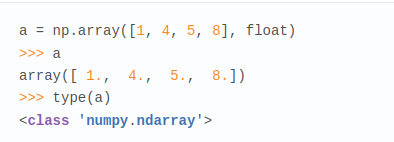
\includegraphics[width=0.5\textwidth,height=0.35\textheight]{pictures/array.png}
  \caption{Об'єкт array}
\label{function}
  \end{center}
\end{figure}
\end{frame}

\begin{frame}
\frametitle{NumPy: методи масивів}
\begin{itemize}
  \item Метод \texttt{a.shape} повертає кількість рядків та стовпців в матриці \texttt{a}.
  \item Метод \texttt{a.dtype} повертає тип змінних, що зберігаються в масиві \texttt{a}.
  \item Метод \texttt{a.fill(n)} заповнює масив \texttt{a} значенням \texttt{n}.
  \item Метод \texttt{a.reshape((n,m))} перетворює масив \texttt{a} у масив розміром \texttt{(n,m)}.
  \item Функція \texttt{np.concatenate(a,b,[c, axis=n])} поєднує матриці \texttt{a} та \texttt{b} (та можливо інші) за розмірністю \texttt{n}.
\end{itemize}

\end{frame}

\begin{frame}
\frametitle{NumPy: методи масивів}
\begin{itemize}
  \item Функція \texttt{np.zeros(s)} (\texttt{np.ones(s)}) створіює матрицю із нулів (одиниць), розмірність задається кортежем \texttt{s}.
  \item Функція \texttt{np.eye(n, k=m)} створіює квадратну матрицю розмірністю \texttt{n} із одиницями по   \texttt{m}-ій діагоналі.
  \item Стандратні операції +, -, *, /, \%, **, математичні функції \texttt{abs}, \texttt{sign}, \texttt{sqrt}, \texttt{log}, \texttt{log10}, \texttt{exp}, тригонометричні функції та оператори \texttt{floor},  \texttt{ceil}  застосовуються до масивів поелементно.
  \item Включено важливі математичні константи \texttt{np.pi} та \texttt{np.e}.

\end{itemize}

\end{frame}

\subsubsection{Пакет SciPy}
\begin{frame}
\frametitle{Можливості SciPy}
\begin{table}
  \caption{Модулі SciPy}
  \label{tab:}

  \begin{center}
    \begin{tabular}{|c|c|}
    \hline
      \textbf{Модуль} & \textbf{Використання} \\
      \hline
      scipy.constants & Математичні та фізичні константи\\
      \hline
      scipy.special & Спеціальні функції математичної фізики\\
      \hline
      scipy.integrate & Чисельне інтегрування\\
      \hline
      scipy.optimize & Максимум/мінімум користувацьких функції\\
      \hline
      scipy.linalg & Функції лінійної алгебри\\
      \hline
    \end{tabular}
  \end{center}
\end{table}
\end{frame}

\begin{frame}
\frametitle{Можливості SciPy}
\begin{table}
  \caption{Модулі SciPy}
  \label{tab:}

  \begin{center}
    \begin{tabular}{|c|c|}
    \hline
      \textbf{Модуль} & \textbf{Використання} \\
      \hline
      scipy.sparse & Робота з розрідженими матрицями\\
      \hline
      scipy.interpolate & Методи та класи для інтерполяції\\
      \hline
      scipy.fftpack & Обробка перетворень Фур'є\\
      \hline
      scipy.signal & Обробка сигналів\\
      \hline
      scipy.stats & Статистичні функції та розподіли\\
      \hline
    \end{tabular}
  \end{center}
\end{table}
\end{frame}

\subsubsection{Пакет Matplotlib}
\begin{frame}
\frametitle{Matplotlib}
Matplotlib - пакет для побудови графіків. Використання:

\texttt{import matplotlib.pyplot as plt}

\begin{figure}
  \begin{center}
    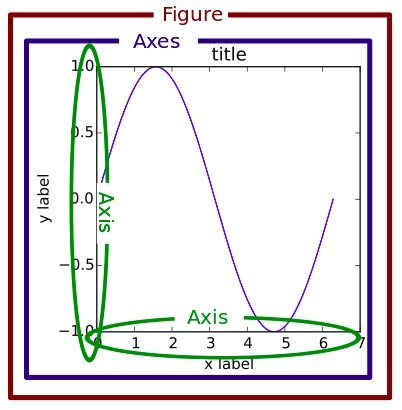
\includegraphics[width=0.5\textwidth,height=0.5\textheight]{pictures/figure-matplotlib.jpg}
  \caption{Ієрархія об'єктів matplotlib}
\label{function}
  \end{center}
\end{figure}
\end{frame}

\begin{frame}
\frametitle{<<Анатомія>> малюнку в Matplotlib}

\begin{figure}
  \begin{center}
    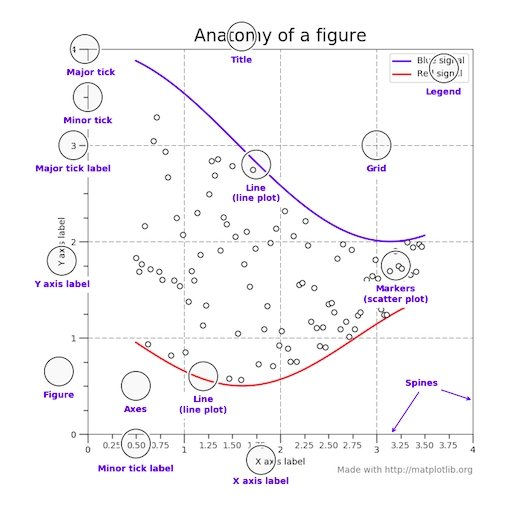
\includegraphics[width=0.6\textwidth,height=0.7\textheight]{pictures/anatomy-matplotlib.jpg}
  \caption{Ієрархія об'єктів matplotlib}
\label{function}
  \end{center}
\end{figure}
\end{frame}

\begin{frame}
\frametitle{Matplotlib: приклад}
\scriptsize
import numpy as np

import matplotlib.pyplot as plt

rng = np.arange(50)

rnd = np.random.randint(0, 10, size=(3, rng.size))

yrs = 1950 + rng

fig, ax = plt.subplots(figsize=(5, 3))

ax.stackplot(yrs, rng + rnd, labels=['Eastasia', 'Eurasia', 'Oceania'])

ax.set\_title('Combined debt growth over time')

ax.legend(loc='upper left')

ax.set\_ylabel('Total debt')

ax.set\_xlim(xmin=yrs[0], xmax=yrs[-1])

fig.tight\_layout()

plt.show()
\normalsize
\end{frame}

\begin{frame}
\frametitle{Matplotlib: приклад}
\begin{itemize}
  \item Після створення трьох часових стовпців (рядів) визначено фігуру (\texttt{fig}), що містить об'єкт \texttt{Axes} (\texttt{plot, ax});
  \item Методи \texttt{ax} викликаються для створення діаграми з розбивкою по областях та додаванням легенди, заголовка та ярлика вісі \texttt{y};
  \item \texttt{tight\_layout()} застосовується до об'єкта Figure для очищення прогалин.
\end{itemize}
\end{frame}

\begin{frame}
\frametitle{Matplotlib: приклад}

\begin{figure}
  \begin{center}
    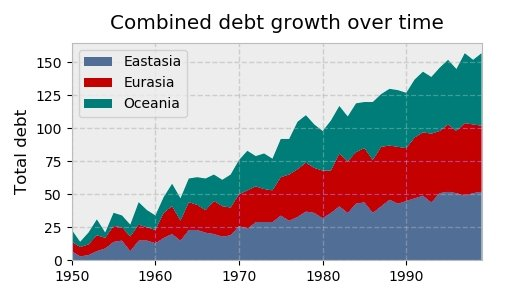
\includegraphics[width=0.6\textwidth,height=0.6\textheight]{pictures/example-matplotlib.jpg}
  \caption{Приклад малюнку в matplotlib}
\label{function}
  \end{center}
\end{figure}
\end{frame}


\end{document}
